\documentclass{article}

% if you need to pass options to natbib, use, e.g.:
%     \PassOptionsToPackage{numbers, compress}{natbib}
% before loading neurips_2018

% ready for submission
\usepackage{neurips_2018}

% to compile a preprint version, e.g., for submission to arXiv, add add the
% [preprint] option:
    % \usepackage[preprint]{neurips_2018}

% to compile a camera-ready version, add the [final] option, e.g.:
     % \usepackage[final]{neurips_2018}

% to avoid loading the natbib package, add option nonatbib:
%     \usepackage[nonatbib]{neurips_2018}

\usepackage[utf8]{inputenc} % allow utf-8 input
\usepackage[T1]{fontenc}    % use 8-bit T1 fonts
\usepackage{hyperref}       % hyperlinks
\usepackage{url}            % simple URL typesetting
\usepackage{booktabs}       % professional-quality tables
\usepackage{amsfonts}       % blackboard math symbols
\usepackage{nicefrac}       % compact symbols for 1/2, etc.
\usepackage{microtype}      % microtypography\usepackage{times}

\usepackage{epsfig}
\usepackage{graphicx}
\usepackage{amsmath}
\usepackage{amssymb}

\usepackage{algorithm}% http://ctan.org/pkg/algorithm
\PassOptionsToPackage{noend}{algpseudocode}% comment out if want end's to show
\usepackage{algpseudocode}% http://ctan.org/pkg/algorithmicx

\makeatletter
\newcommand*{\skipnumber}[2][1]{%
   {\renewcommand*{\alglinenumber}[1]{}\State #2}%
   \addtocounter{ALG@line}{-#1}}
\makeatother

% \newcommand*{\algrule}[1][\algorithmicindent]{\makebox[#1][l]{\hspace*{.5em}\vrule height .75\baselineskip depth .25\baselineskip}}%

% \newcount\ALG@printindent@tempcnta
% \def\ALG@printindent{%
%     \ifnum \theALG@nested>0% is there anything to print
%         \ifx\ALG@text\ALG@x@notext% is this an end group without any text?
%             % do nothing
%             \addvspace{-3pt}% FUDGE for cases where no text is shown, to make the rules line up
%         \else
%             \unskip
%             % draw a rule for each indent level
%             \ALG@printindent@tempcnta=1
%             \loop
%                 \algrule[\csname ALG@ind@\the\ALG@printindent@tempcnta\endcsname]%
%                 \advance \ALG@printindent@tempcnta 1
%             \ifnum \ALG@printindent@tempcnta<\numexpr\theALG@nested+1\relax% can't do <=, so add one to RHS and use < instead
%             \repeat
%         \fi
%     \fi
%     }%
\usepackage{etoolbox}
% the following line injects our new indent handling code in place of the default spacing
% \patchcmd{\ALG@doentity}{\noindent\hskip\ALG@tlm}{\ALG@printindent}{}{\errmessage{failed to patch}}
% \makeatother
% end vertical rule patch for algorithmicx

\usepackage{tabularx}
\usepackage{lipsum}
\usepackage{makecell}
\usepackage{multirow}
\usepackage[labelformat=simple]{subcaption}
\renewcommand\thesubfigure{(\alph{subfigure})}
\usepackage{booktabs}

\newcommand*{\cost}{c}%
\newcolumntype{M}[1]{>{\centering\arraybackslash}m{#1}}
% \newcolumntype{M}[1]{>{\arraybackslash}m{#1}}

% Include other packages here, before hyperref.

% If you comment hyperref and then uncomment it, you should delete
% egpaper.aux before re-running latex.  (Or just hit 'q' on the first latex
% run, let it finish, and you should be clear).
% \usepackage[pagebackref=true,breaklinks=true,letterpaper=true,colorlinks,bookmarks=false]{hyperref}

% \iccvfinalcopy % *** Uncomment this line for the final submission

\def\iccvPaperID{368} % *** Enter the ICCV Paper ID here
\def\httilde{\mbox{\tt\raisebox{-.5ex}{\symbol{126}}}}


\DeclareMathOperator*{\argmax}{arg\,max}
\DeclareMathOperator*{\argmin}{arg\,min}
\usepackage{mathrsfs}
\newcommand{\RED}[1]{#1}

\newcommand\TODO[1]{{\color{red}{TODO: #1}}}
\newcommand\UPDATE[1]{{\color{blue}{#1}}}
\newcommand\SOURCE[1]{{\color{green}{(from: #1)}}}
% \newcommand\CHANGED[2]{{{\color{blue}{#1}}\color{green}{#2}}}

\usepackage[dvipsnames]{xcolor}
\usepackage[shortlabels]{enumitem}


%%%%%%%%% TITLE
\title{Generalized Framework for \\Agglomerative Clustering of Signed Graphs \\applied to bottom-up instance segmentation}

% The \author macro works with any number of authors. There are two commands
% used to separate the names and addresses of multiple authors: \And and \AND.
%
% Using \And between authors leaves it to LaTeX to determine where to break the
% lines. Using \AND forces a line break at that point. So, if LaTeX puts 3 of 4
% authors names on the first line, and the last on the second line, try using
% \AND instead of \And before the third author name.

\author{%
  David S.~Hippocampus\thanks{Use footnote for providing further information
    about author (webpage, alternative address)---\emph{not} for acknowledging
    funding agencies.} \\
  Department of Computer Science\\
  Cranberry-Lemon University\\
  Pittsburgh, PA 15213 \\
  \texttt{hippo@cs.cranberry-lemon.edu} \\
  % examples of more authors
  % \And
  % Coauthor \\
  % Affiliation \\
  % Address \\
  % \texttt{email} \\
  % \AND
  % Coauthor \\
  % Affiliation \\
  % Address \\
  % \texttt{email} \\
  % \And
  % Coauthor \\
  % Affiliation \\
  % Address \\
  % \texttt{email} \\
  % \And
  % Coauthor \\
  % Affiliation \\
  % Address \\
  % \texttt{email} \\
}
\begin{document}

\maketitle
%\thispagestyle{empty}



% !TEX root = ../agglo_clust_review.tex
%%%%%%%%% ABSTRACT
\begin{abstract}
We propose a new simple theoretical framework that generalizes algorithms for hierarchical agglomerative clustering to weighted graphs with both attractive and repulsive interactions between the nodes. This framework defines GASP, a Generalized Algorithm for Signed graph Partitioning, and allows us to explore many combinations of different linkage criteria and cannot-link constraints. 
We prove the equivalence of existing clustering methods to some of those combinations, and introduce new algorithms for combinations which have not been studied before. 
We also study theoretical properties of these combinations and prove which one of them define ultrametrics on the graph.
% On stochastic block model problems, GASP compares favorably to spectral clustering. 
We conduct a systematic comparison of various instantiations of GASP on a large variety of both synthetic and existing signed clustering problems, in terms of accuracy but also efficiency and robustness to noise. 
More importantly, we find that some of the algorithms proposed in our framework, when combined to the predictions from a CNN model, result in a simple instance segmentation pipeline that achieves state-of-the-art performances on the competitive CREMI 2016 EM segmentation benchmark.
% \keywords{Partitioning of Signed Graphs, Generalized Framework, Agglomerative Clustering, Instance Segmentation}
\end{abstract}


% !TEX root = ../agglo_clust_review.tex

\section{Introduction}
%On possible selling story could be: currently many of the successful proposal-free instance segmentation methods rely on a final clustering step on a grid-graph with both short and long-range connections. So it is worth to study this problem in more details. 

Deep convolutional neural nets (CNNs) has been successfully applied to a wide range of tasks of computer vision and pixel-level image understanding, such as \UPDATE{boundary detection \cite{arbelaez2011contour,xie2015holistically,maninis2018convolutional}, semantic segmentation \cite{long2015fully,chen2018deeplab,kong2018recurrent}, optical flow \cite{weinzaepfel2013deepflow,dosovitskiy2015flownet}, and pose estimation \cite{wei2016convolutional,cao2017realtime}.}


\begin{itemize}
% \SOURCE{\cite{kong2018recurrent}}
\item \emph{Instance segmentation} is a task of computer vision that involves the detection of all objects in an image by performing pixel-level segmentation of each instance.   
\item Many recent successful methods for instance segmentation %, usually named \emph{proposal-based methods}, 
 use heuristic approaches that start from the classical computer vision task of \emph{object detection}, where the goal is to localize each objects using a bounding box, and then predict both a pixel-level mask of each instance and a semantic label (classify the objects in the bounding box). \TODO{Is it really general enough as a description...?} \cite{yang2012layered,ladicky2010and,hariharan2014simultaneous,chen2015multi,dai2016instance,liang2016reversible,he2017mask}
\item While effective, these approaches are \UPDATE{somewhat unsatisfying (copy/paste, change: present some faults)} because:
\begin{itemize}
\item they rely on the object detector and non-maximum suppression heuristics to count how many instances are present in the image, 
\item they tend to underperform in cluttered scenes, since instance assignment is often carried out independently for each detection; 
\item they are not usable for wiry or articulated objects (e.g. in the field of connectomics and neuron segmenation from electron microscopy images) 
\item their architecture do not usually prevent a pixel to be shared between multiple instances
\item they do not scale up well since each proposal has to be singularly processed by the CNN. 
% \item (difficult to train in an end-to-end manner: interface between instance segmentation and detection is non-differentiable)
% \item (architecture is complex and hard to tune and “debug”...?)
\end{itemize}

\item Currently there are two successful approaches used for proposal-free instance segmentation: the first ones predict associative pixel embedding vectors, where the goal is to have a CNN predicting embedding vectors that are similar only for pixels in the same instance \cite{kong2018recurrent,fathi2017semantic,newell2017associative,de2017semantic}; in the second type of approaches, for every pixel a set of neighboring pixels is fixed  (not necesarelly limited to the direct neighbors) and a CNN then predicts affinities, that represent how likelity it is for each of neighboring pixels to be in the same instance \cite{liu2018affinity,wolf2018mutex,xie2015holistically}

\item Both approaches requires a final clustering algorithm to output the final instance segmentation 

 and we can define a grid graph, where each vertex represents a pixel, with short- and long-range edge connections 

 and find the final instance segmentation by using a graph clustering algorithm.

\item Recent work (\cite{wolf2018mutex}, more...) shows that it is better to use \textbf{repulsion and attraction} (directly predict it with the classifier, no need to define seeds or to fix a threshold given an hierarchy of clusters)
\item solving correlation clustering problem (multicut) is too expensive for this application (even using recently proposed heuristics)
\item our contributions:
\begin{itemize}
\item we propose a unified and simple formalization of Agglomerative Clustering and show how many of the recently proposed methods can be seen as special cases (focusing in particular on signed graphs) (\textbf{review and comparison paper})
\item new clustering algorithms on signed graphs
\item we compare different types of agglomeration clustering on a pixel grid graph with short and long-range connections, focusing on aspects like efficieny, robustness (and MC energy) 

\end{itemize}
\item on other datasets (connectomics) many methods are based on multi-step pipelines first predicting superpixels
\item \textit{if we get good scores on CREMI}: we show that also on neuro-data it is worth to skip the hand-crafted superpixel step and compute the final segmentation directly from the CNN affinities (MWS already showed it on the ISBI dataset)

\end{itemize}


\begin{figure}[t]
\centering
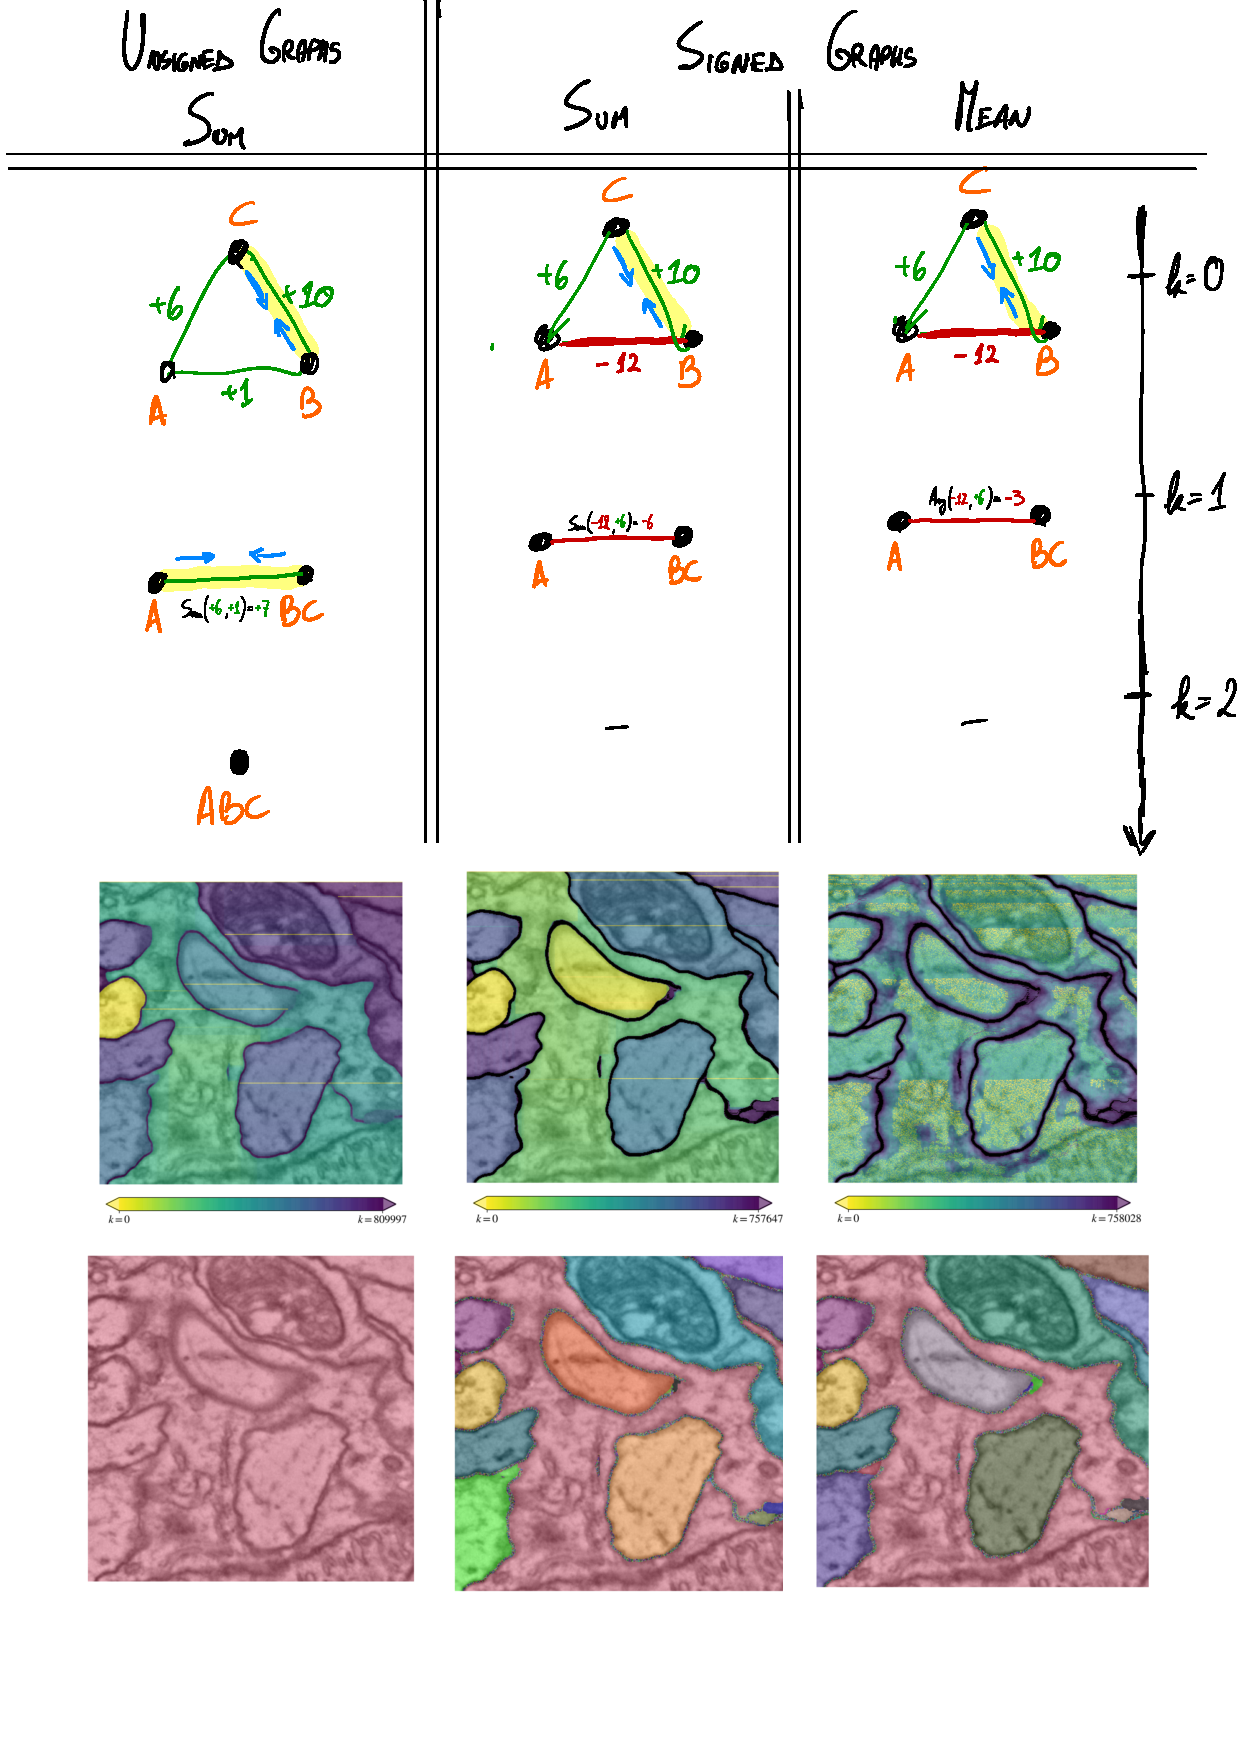
\includegraphics[width=\textwidth,trim=0.4in 1.2in 0.in 0.05in,clip]{./figs/intro_image.jpg} % left bottom right top
\caption{\small 
Intro image: explain algorithm, main ideas and contributions
\label{fig:intro_figure}}
\end{figure}


% !TEX root = ../agglo_clust_review.tex

\section{Related work}

% \begin{itemize}

% \item Contributions: (and mention introductory Figure)
% \begin{itemize}
% \item We generalize the hierarchical agglomerative clustering framework to graphs with positive and negative edge attributes
% \item We review both standard hierarchical clustering algorithms and signed graph partitioning algorithms by showing how they can be described in this simplified framework (and as special cases of the general algorithm presented in Sec. \ref{sec:algorithm})
% \item we introduce and test new variations of these algorithms for signed graphs
% \end{itemize}
% \end{itemize}

% \begin{itemize}
% \item Motivation 2:
% \begin{itemize}
% \item HC has been always really popular in computer vision: \emph{Instance segmentation} is a task of computer vision that involves the detection of all objects in an image by performing pixel-level segmentation of each instance.   
% \item Since conventional unsigned graph agglomerative clustering algorithms, such as the well-known linkage methods [1], usually are quite sensitive to noise and outliers [1] (As their affinities are directly computed using pairwise distances between samples), most methods were based on multi-step pipelines first predicting superpixels (to reduce noise).
% \item These methods are still commonly used for specific instance segmentation applications: connectomics, build merge-tree 
%  %https://arxiv.org/pdf/1208.5092.pdf
% \item still commonly used for building merge-trees, give recent examples in connectomics (Sebastian Seung, etc...) % https://arxiv.org/abs/1608.04051
% \item Graph clustering algorithms recently gained more and more popularity with the advent of deep-learning and its application to instance segmentation
% \item Deep convolutional neural nets (CNNs) has been successfully applied to a wide range of tasks of computer vision and pixel-level image understanding, such as \UPDATE{boundary detection \cite{arbelaez2011contour,xie2015holistically,maninis2018convolutional}, semantic segmentation \cite{long2015fully,chen2018deeplab,kong2018recurrent}, optical flow \cite{weinzaepfel2013deepflow,dosovitskiy2015flownet}, and pose estimation \cite{wei2016convolutional,cao2017realtime}.}
% % \SOURCE{\cite{kong2018recurrent}}

% \item Currently there are two successful approaches used for proposal-free bottom-up instance segmentation: the first ones predict associative pixel embedding vectors, where the goal is to have a CNN predicting embedding vectors that are similar only for pixels in the same instance \cite{kong2018recurrent,fathi2017semantic,newell2017associative,de2017semantic}; in the second type of approaches, for every pixel a set of neighboring pixels is fixed  (not necesarelly limited to the direct neighbors) and a CNN then predicts affinities, that represent how likely it is for each of neighboring pixels to be in the same instance \cite{liu2018affinity,wolf2018mutex,xie2015holistically}

% \item Both approaches requires a final clustering algorithm to output the final instance segmentation 

%  and we can define a grid graph, where each vertex represents a pixel, with short- and long-range edge connections 

%  and find the final instance segmentation by using a graph clustering algorithm.

% \item GMIS achieved 
% comparable results to methods based on object 
% proposal like Mask-R-CNN on natural images 
% (Cityscapes); MWS achieved SOA results on a 
% biological images (ISBI)

% \item Out contributions:

% \begin{itemize}
%  \item we compare different types of agglomeration clustering on a pixel grid graph with short and long-range connections, focusing on aspects like efficieny, robustness (and quality of the final clustering in terms of multicut energy) \textbf{Comparison paper}
%  \item \textit{if we get good scores on CREMI dataset}: we show that also on neuro-data it is worth to skip the hand-crafted superpixel step and compute the final segmentation directly from the CNN affinities (MWS already showed it on the ISBI dataset): main selling point is again the almost-parameter free feature of the method
% \end{itemize}
% \end{itemize}
% \end{itemize}


% More details about instance segmentation (move to related work)
% \begin{itemize}


% \item 
% \item Many recent successful methods for instance segmentation %, usually named \emph{proposal-based methods}, 
%  use heuristic approaches that start from the classical computer vision task of \emph{object detection}, where the goal is to localize each objects using a bounding box, and then predict both a pixel-level mask of each instance and a semantic label (classify the objects in the bounding box). \TODO{Is it really general enough as a description...?} \cite{yang2012layered,ladicky2010and,hariharan2014simultaneous,chen2015multi,dai2016instance,liang2016reversible,he2017mask}
% \item While effective, these approaches are \UPDATE{somewhat unsatisfying (copy/paste, change: present some faults)} because:
% \begin{itemize}
% \item they rely on the object detector and non-maximum suppression heuristics to count how many instances are present in the image, 
% \item they tend to underperform in cluttered scenes, since instance assignment is often carried out independently for each detection; 
% \item they are not usable for wiry or articulated objects (e.g. in the field of connectomics and neuron segmenation from electron microscopy images) 
% \item their architecture do not usually prevent a pixel to be shared between multiple instances
% \item they do not scale up well since each proposal has to be singularly processed by the CNN. 
% % \item (difficult to train in an end-to-end manner: interface between instance segmentation and detection is non-differentiable)
% % \item (architecture is complex and hard to tune and “debug”...?)
% \end{itemize}

% \item Currently there are two successful approaches used for proposal-free (make brief intro) instance segmentation: the first ones predict associative pixel embedding vectors, where the goal is to have a CNN predicting embedding vectors that are similar only for pixels in the same instance \cite{kong2018recurrent,fathi2017semantic,newell2017associative,de2017semantic}; in the second type of approaches, for every pixel a set of neighboring pixels is fixed  (not necesarelly limited to the direct neighbors) and a CNN then predicts affinities, that represent how likely it is for each of neighboring pixels to be in the same instance \cite{liu2018affinity,wolf2018mutex,xie2015holistically}

% \item Both approaches requires a final clustering algorithm to output the final instance segmentation 

%  and we can define a grid graph, where each vertex represents a pixel, with short- and long-range edge connections 

%  and find the final instance segmentation by using a graph clustering algorithm.

% \item Recent work (\cite{wolf2018mutex}, more...) shows that it is better to use \textbf{repulsion and attraction} (directly predict it with the classifier, no need to define seeds or to fix a threshold given an hierarchy of clusters)
% \item solving correlation clustering problem (multicut) is too expensive for this application (even using recently proposed heuristics)
% \item our contributions:
% \begin{itemize}
% \item we propose a unified and simple formalization of Agglomerative Clustering and show how many of the recently proposed methods can be seen as special cases (focusing in particular on signed graphs) (\textbf{review and comparison paper})
% \item new clustering algorithms on signed graphs


% \end{itemize}
% \item on other datasets (connectomics) many methods are based on multi-step pipelines first predicting superpixels


% \end{itemize}


\begin{itemize}

% \item \emph{Possible intro about aggl. clustering:} \UPDATE{Hierarchical, agglomerative clustering is an important and well-established technique in unsupervised machine learning. Agglomerative clustering schemes start from the partition of the data set into singleton nodes and merge step by step the current pair of mutually closest nodes into a new node until there is one final node left, which comprises the entire data set. Various clustering schemes share this procedure as a common definition, but differ in the way in which the measure of inter-cluster dissimilarity is updated after each step. } %\cite{mullner2011modern}



% \item \emph{Other possible intro:} Many problems in computer vision involve clustering. Partitional clustering, such as k-means [1], determines all clusters at once, while agglomerative clustering [1] begins with a large number of small clusters, and iteratively selects two clusters with the largest affinity under some measures to merge, until some stopping condition is reached. Ag- glomerative clustering has been studied for more than half a century, and used in many applications [1], because it is conceptually simple and produces an informative hierar- chical structure of clusters. % FROM https://arxiv.org/pdf/1208.5092.pdf#page14

% \item Get more specific about graph (we do not cluster points in a space, but we cluster vertices with specified neighbors and interactions given by edges). 

% \item HC is a popular graph partitioning algorithm. Why: more efficient than divisive approaches and graph cuts; does not usually require to specify the final number of clusters (e.g. spectral clustering) or seed nodes (e.g. watershed, random walker). \UPDATE{And if the graph is not dense, HC algorithms scale up well with complexity}

% \item Motivation 1:

% \begin{itemize}

% \item all HC methods only talk about positive edge weights, but it is actually easy to generalize them for negative and attractive edges. 
% \item The standard version of HC is good for building hierarchy but problem with hierarchical merge-trees is how to choose one single threshold. Choose one single fixed density level. Ideally we would like to be able to cut the tree at different places to select our clusters.
% \item An important line of research is based on the observation that superior partitionings are obtained when the graph has both attractive and repulsive edges. Solutions that optimally balance attraction and repulsion do not require external stopping criteria such as predefined number of regions or seeds. This generalization leads to the NP-hard problem of correlation clustering or (synonymous) multicut (MC) partitioning. \emph{Alternative:} multicut / correlation clustering partitions vertices with both attractive and repulsive interactions encoded into the edges of a graph. Multicut has the great advantage that a “natural” partitioning of a graph can be found, without needing to specify a desired number of clusters, or a termination criterion, or one seed per region. Its great drawback is that its optimization is NP-hard.

% \end{itemize}



\item \textbf{Proposal based methods} 
\begin{itemize}
\item Generate region proposals or bounding boxes and classify the objects in the bounding box \cite{yang2012layered,ladicky2010and,hariharan2014simultaneous,chen2015multi,dai2016instance,liang2016reversible,he2017mask}; fully convolutional  box proposals \cite{li2017fully}. 
\item \emph{More references:} or generate generic proposal segments and then label each one with a semantic detector \cite{hariharan2014simultaneous,chen2015multi,hariharan2015hypercolumns,dai2015convolutional,uhrig2016pixel,he2017mask}.
\item these somehow still uses some kind of object detector (at least to find the number of objects), but they do not necessary analyse one proposal at the time: use an object detector to enumerate candidate instances and then perform pixel-level segmentation of each instance \cite{liang2018proposal,dai2016instance,li2017fully,liang2016reversible,arnab2017pixelwise} \TODO{check \cite{dai2016instance}}
% \SOURCE{\cite{kong2018recurrent}
\end{itemize}

\item \textbf{Proposal-free methods:} 
\begin{itemize}
\item box-free \cite{pinheiro2015learning,pinheiro2016learning,hu2017fastmask}; joint segmentation and instance labeling in a combinatorial framework \cite{kirillov2017instancecut}; recurrent models \cite{romera2016recurrent,ren2017end}; encode instance relationships to classes and exploit the boundary information  \cite{jin2016object}; sequential framework to gradually group from points to lines and then instances \cite{liu2017sgn}
% \item From end-to-end recurrent attention: \textit{Other approaches us- ing FCNs are proposal-free, but rely on a \textbf{bottom-up merging process}\textbf{}. Liang et al. [26] predict dense pixel prediction of ob- ject location and size, using clustering as a post-processing step. Uhrig et al. [41] present another approach based on FCNs, which is trained to produces a semantic segmen- tation as well as an instance-aware angle map, encoding the instance centroids. Post-processing based on template matching and instance fusion produces the instance identi- ties. Importantly, they also used ground-truth depth labels in training. Concurrent work [2, 19, 22] also explores a similar idea of using FCNs to output instance-sensitive embeddings.}
\item \textbf{Pixel embedding vectors}: 
\begin{itemize}
\item supervised vectors \cite{bai2017deep}, unsupervised vectors  \cite{kong2018recurrent,fathi2017semantic,newell2017associative,de2017semantic} of which \cite{kong2018recurrent} is trained end-to-end;  using scene depth information \cite{uhrig2016pixel}, \TODO{check \cite{sironi2014multiscale}} 
%    \TODO{more on pose estimation, vector distance transform, deep coloring?, ECCV semi-convolutions}

% different types of loss
% \item For each pixel in the image, a CNN predicts an embedding vector, such that pixels in the same instance are represented by the same vector. (\textit{by training a model that labels pixels with unit-length vectors that live in some fixed dimension embedding space} \SOURCE{Rec. embeddings} ). \textit{With instance embedding, each object is assigned a “color” in a n-dimensional space. The network processes the image and produces a dense output, same size as the input image. Each pixel in the output of the network is a point in the embedding space. Pixels that belong to the same object are close in the embedding space while pixels that belong to different objects are distant in the embedding space. Parsing the image embedding space involves some sort of clustering algorithm.} \SOURCE{online} 

% \item Clustering methods: DBSCAN, more

\item \emph{Division by used clustering methods}: spectral clustering \cite{liang2018proposal}; mean-shift \cite{kong2018recurrent}; HDBSCAN \cite{}; seeds \cite{fathi2017semantic} \TODO{incomplete}
\end{itemize}

% \item Nevertheless, in both approaches we can define a grid graph (each vertex representing a pixel) with signed weights and find the final instance segmentation by using a graph partitioning algorithm:
% \begin{itemize}
% \item In Method 1, the graph is complete and the edge weights represent similarities between pairs of pixel embedding vectors. In most proposed approaches, embedding vectors representing distinct instances should be "distant enough" in the embedding space (a minimum distance is usually used during the training of the CNN). Thus, this threshold distance can be used to define signed affinities, representing attraction or repulsion between pairs of pixels;
% \item  In Method 2, the short- and long-range affinities predicted by the CNN are directly used as signed edge weights in the grid graph
% \end{itemize}



\item \textbf{Most related: predict short- and long-range affinities}. For each pixel we fix a set of neighboring pixels (not necessarily limited to the direct neighbors) and CNN predicts how likely it is for each pixel pair to be in the same instance \cite{liu2018affinity,wolf2018mutex,lee2017superhuman,xie2015holistically,Maire_2016_CVPR}. Mention that  \cite{liu2018affinity} is SoA on cityscapes for proposal-free methods and \cite{wolf2018mutex} is SoA on ISBI
% \item \cite{liu2018affinity} achieved comparable results to methods based on object proposal like Mask-R-CNN on natural images (Cityscapes); \cite{wolf2018mutex} achieved SOA results on a biological images (ISBI)
% \item Side comment: Even with pixel embedding vectors we can deduce affinities or signed costs
% (see MWS paper for a good review)

\end{itemize}



\item \textbf{Graph clustering related work}:
\begin{itemize}
    \item popular in image segmentation: \textbf{agglomerative clustering}.
    \item {\small More from \cite{mullner2011modern}: The seven most common methods are termed single, complete, average (UPGMA), weighted (WPGMA, McQuitty), Ward, centroid (UPGMC) and median (WPGMC) linkage (see Everitt et al., 2011, Table 4.1). They are implemented in standard numerical and statistical software such as R (R Development Core Team, 2011), MATLAB (The MathWorks, Inc., 2011), Mathematica (Wolfram Research, Inc., 2010), SciPy (Jones et al., 2001).}
    \item Why: more efficient than divisive approaches and graph cuts; does not usually require to specify the final number of clusters (e.g. spectral clustering) or seed nodes (e.g. watershed, random walker) 
    % old graph cut paper: \cite{shi2000normalized}
    % \item \emph{[other clustering methods working in an euclidean embedding space like mean-shift, K-means, Mixture models, BIRCH... can most probably be omitted]}
    \item many segmentation pipelines used to start the agglomeration from superpixels (SLIC, \cite{felzenszwalb2004efficient}, watershed) to reduce size of the problem 
    \item usually we build an hierarchy of clusters (or a \emph{merge-tree}): \TODO{find meaningful order}
    \item clustering paper suggested by Roman; Cocoons

 
% \item \textit{Some reference (atm in random order, to be continued)} 
\begin{itemize}

\item examples on natural images \cite{ren2013image,liu2016image}; ultra-metric contour map \cite{arbelaez2011contour};
\item \emph{Linkage criteria}: arithmetic average \cite{liu2018affinity,lee2017superhuman}; 
quantiles (median) \cite{funke2018large}; % and structured training 
   learned linkage criteria \cite{nunez2013machine}; 
\item An optimization perspective is taken in \cite{kiran2014global} %, which introduces h-increasing energy functions and builds the hierarchy incrementally such that merge decisions greedily minimize the energy
% Check MWS for description and more details
\item normalized cuts and combinatorial grouping \cite{arbelaez2014multiscale}
\item In \emph{connectomics}: \cite{liu2016sshmt}. Use loopy graphs \cite{kaynig2015large,krasowski2015improving} or trees \cite{liu2016sshmt,liu2014modular,funke2015learning,uzunbas2016efficient} to represent the region merging hierarchy. Using local \cite{liu2014modular,krasowski2015improving} or structured \cite{funke2015learning,uzunbas2016efficient} learning based methods % \SOURCE{SSHMT} Check Funke proposals
\end{itemize}
\item Methods finding a flat clustering (no hierarchy): efficient Graph-based Image segmentation \cite{felzenszwalb2004efficient} % defines a measure of quality for the current regions and stops when the merge costs would exceed this measure
\item \textbf{Signed graphs} \TODO{more}
\begin{itemize}
    % \item problem with hierarchical merge-trees is how to choose one single threshold. Choose one single fixed density level. Ideally we want to be able to cut the tree at different places to select our clusters. In density space, \cite{campello2013density}
    \item Multicut pipiline and heuristics \cite{beier2017multicut}... 
    % \item \textit{\textbf{Multicut} has the great advantage that a “natural” partitioning of a graph can be found, without needing to specify a desired number of clusters, or a termination criterion, or one seed per region. Its great drawback is that its optimization is NP-hard.} \SOURCE{MWS}.

\item hierarchy and multicut proposals \cite{funke2018candidate}
\item \textit{Must-not-link edges:} initially introduced as hard-constraints \cite{malmberg2011generalized}, then introduced dynamically \cite{wolf2018mutex,levinkov2017comparative}. 
\item Local-search approximations of MC: greeedy fixation and greedy additive edge contraction \cite{levinkov2017comparative}
\end{itemize}
\end{itemize}

\end{itemize}



% !TEX root = ../agglo_clust_review.tex

\section{Generalized framework for agglomerative clustering of signed graphs} \label{sec:general_framework}
% In this section, we first define notation and then introduce one of our main contributions: a signed graph partitioning algorithm (Sec. \ref{sec:algorithm}) that can be seen as a generalization of several existing and new clustering algorithms (Sec. \ref{sec:alg_update_rules}).

\subsection{Notation} \label{sec:notation}

\textbf{Graph formalism} -- We consider an undirected simple edge-weighted graph $\mathcal{G}(V,E,w^+, w^-)$ with both attractive and repulsive edge attributes.
% In computer vision applications, the nodes can represent either pixels, superpixels or voxels.  
The weight function $w^+: E \rightarrow \mathbb{R}^+$ associates to every edge a positive scalar attribute $w_e^+\in \mathbb{R}^+$ representing a merge affinity or a similarity measure.
% the higher this number, the higher the inclination of the two incident vertices to be assigned to the same cluster\footnote{Note that other formalisms for positively weighted graphs associate distances to the edges, thus, the \emph{lower} the edge weight, the higher the attraction between the two linked nodes, contrary to our definition of $w^+$.}. 
On the other hand, $w^-: E \rightarrow \mathbb{R}^+$ associates to each edge a split tendency $w_e^- \in \mathbb{R}^+$: \OPTIONAL{the higher this number, the higher the inclination of the two incident vertices to be assigned to different clusters}.
% the higher this weight, the more the incident vertices would like to be in different clusters. 
Graphs of the type $\mathcal{G}(V,E,w^+, w^-)$ are often defined as \emph{signed graphs} $\mathcal{G}(V,E,\cost)$, featuring positive and negative edge weights $\cost_e\in \mathbb{R}$. Following the theoretical considerations in \cite{lange2018partial}, we define these signed weights as ${\cost_e = w_e^+ - w_e^-}$. 
% Some approaches directly compute $\cost_e$, whereas others compute $w_e^+$ and $w_e^-$ separately.
% In this formalism, graphs with purely attractive interactions are a special case of $\mathcal{G}(V,E,\cost)$ with $\cost_e \geq 0, \, \forall e \in E$. 

\textbf{Multicut objective} -- We call the set $\Pi$ a \emph{clustering} or \emph{partitioning} with $K$ clusters if $V = \cup_{S\in\Pi} S $, $\,S \cap S' = \emptyset$ for different clusters $S, S'\in \Pi$ and every cluster $S \in \Pi$ induces a connected subgraph of $\mathcal{G}$. 
For any clustering $\Pi$ of $\mathcal{G}$, we define as $E^0_\Pi= \{ e_{uv} \in E \,|\, \exists S \in \Pi : u,v \in S \}$ the set of edges linking nodes in the same cluster, and as $E_\Pi^1= E \setminus E^0_\Pi$ the set of edges whose linked nodes belong to distinct clusters.
% \begin{equation}
% E_\Pi^0 \equiv \{ e_{uv} \in E \,|\, \exists S \in \Pi : u \in S \, \text{and} \, v \in S \}, \qquad E^1_\Pi \equiv E \setminus E^0_\Pi.
% \end{equation}
% \begin{align}
% E_\Pi^0 &= \{ e_{uv} \in E \,|\, \exists S \in \Pi : u \in S \, \text{and} \, v \in S \}, \\
% E^1_\Pi &= E \setminus E^0_\Pi.
% \end{align}
The set of edges $E_\Pi^1$ is known as the \emph{multicut} of $\mathcal{G}$ associated to clustering $\Pi$. The instance of the NP-hard \emph{minimum cost multicut problem} w.r.t. $\mathcal{G}(V,E,w_e)$ is the task of finding a clustering that optimally balance the attraction and repulsion in the graph and is given by the following binary integer program:
\begin{equation}
% \min_\Pi \texttt{MC}(\Pi) \equiv
 \min_\Pi \sum_{e\in E} \cost_e x_e^\Pi,  \qquad \text{where} \quad x^\Pi_e = 
 \begin{cases} 
 1 & \text{if } e\in E^1_\Pi \\
 0 & \text{otherwise}.
 \end{cases}
\end{equation}
% In the next chapters we will use this objective as a way to measure how balanced is a clustering found by the tested agglomerative clustering algorithms.


\textbf{Weight-shift hierarchical algorithms} -- Given an algorithm that outputs a clustering $\Pi$ for a signed graph $\mathcal{G}(V,E,w_e)$, we call the algorithm \emph{weight-shift hierarchical} if, by adding a constant $\alpha \in \mathbb{R}$ to all edge weights $w_e$, the algorithm outputs a clustering $\Pi'$ which is a coarsening of $\Pi$ when $\alpha>0$ and a refinement of $\Pi$ when $\alpha<0$\footnote{A clustering $\Pi'$ is a coarsening of $\Pi$ when every $S' \in \Pi'$ is the union of one or more clusters in $\Pi$. Similarly, $\Pi'$ is a refinement of $\Pi$ when every $S \in \Pi$ is given by the union of one or more clusters in $\Pi'$}.

\textbf{Linkage criteria and hierarchical trees} -- 
% We also denote as $S_u$ the cluster associated with node $u$ \TODO{Needed?}.
% We call two clusters $S,S'$ \emph{adjacent} if there exists at least one edge ${e_{ts}\in E}$ connecting a node $t\in S_u$ to a node $s\in S_v$. 
Let the interaction $\interact(S,S')$ between two clusters $S,S'$ be defined as a function $\interact{}:2^{V} \times 2^{V} \rightarrow \mathbb{R}$, named \emph{linkage criterion}, depending on the weights of \emph{all} edges connecting clusters $S$ and $S'$, i.e. ${(S \times S') \cap E}$. 
The linkage criteria tested in this article are listed and defined in Table \ref{tab:linkage-criteria}.
In hierarchical clustering (HC) literature,  a \emph{dendrogram} $T$ is a rooted binary tree\footnote{In general, one could look at trees that are not binary. However, the algorithms discussed in this paper always generate binary hierarchical trees, so nothing would be gained by this generalization.} representing the merging order of an agglomerative algorithm, such that the leaves of the tree are in one-to-one correspondence with $V$. 
Let $T_{\mathrm{R}},T_{\mathrm{L}}\subset T$ denote the subtrees rooted at the two children of the root node in $T$.
For any two leaves $u,v \in V$, let $T[u \vee v]$ be the subtree rooted at the least common ancestor $u \vee v\in T$ of nodes $u$ and $v$ (furthest from the root), and let \texttt{leaves}$(T[u \vee v])\subseteq V$ be the set of leaves of this subtree. 
% \TODO{Here we talk about the algorithm already, so we could move it to next section and the flow could be better. But we need a tree in the alg. So we better do this later}
% Algorithm \ref{main_alg} returns a binary tree denoted by $T^*$.
Given an agglomerative algorithm with merging tree $T$, let $h_T:T \rightarrow \mathbb{N}$ denote the \emph{dendrogram-height} of each $(u\vee v)\in T$, which is defined as the iteration number at which nodes $u,v\in V$ were merged (\TODO{Fig.~1}). We also define the interaction $\treeHeight(u,v)$ as the interaction $\interact{}(S,S')$ between the two clusters $S,S'$ that were merged at iteration $h_T(u\vee v)$: 
% Then, given a binary tree $T$ and a linkage criterion $\interact$, we can associate a \emph{signed similarity} function $\treeHeight$ to each pair of distinct original nodes $u\neq v$, with $u, v \in V$:
\begin{equation}\label{eq:def_dendr_interact}
\treeHeight(u,v) \equiv \interact{} \big( \text{\texttt{leaves}}(T_{\mathrm{R}}[u \vee v]), \text{\texttt{leaves}}(T_{\mathrm{L}}[u \vee v]) \big)
\end{equation}
% \OPTIONAL{In other words, $h_T(u,v)$ and $\treeHeight(u,v)$ represent the \emph{dendrogram-height} and \emph{signed-interaction} associated to each $u \vee v$ node in the tree $T$ (see toy example in \TODO{Fig.~1}).}




% \begin{algorithm}[t]
%   \caption{\algname{}: generalized algorithm for signed graph partitioning}
%    \hspace*{\algorithmicindent} \textbf{Input:} Graph $\mathcal{G}(V,E,w^+,w^-)$; linkage criterion $\interact{}$; boolean {\color{blue}\texttt{addCannotLinkConstraints}}  \\
%   \hspace*{\algorithmicindent} \textbf{Output:} Final clustering $\Pi$\\
%   \hspace*{\algorithmicindent} 
%   \begin{algorithmic}[1]
%       \State Initialize clustering $\Pi=\{\{v_1\}, \ldots, \{v_{|V|}\}\}$ with each node in its own cluster
%       \State Initial interactions between nodes given by $\cost_e = w^+_e - w^-_e$
%       \Repeat
%         \State Select pair of clusters $S_u,S_v\in\Pi$ with highest absolute interaction $|\interact{}(S_u,S_v)|$
%         \If{\big[{\color{ForestGreen}\textbf{$\interact{}(S_u,S_v) > 0$}}\big] \textbf{and} \big[$S_u,S_v$ are \textbf{not} constrained\big]}
%           \State Merge cluster $S_u$ with $S_v$: update interactions and cannot-link constraints with all their neighbors
%         \ElsIf{\big[{\color{red}\textbf{$\interact{}(S_u,S_v) \leq 0$}}\big] \textbf{and} {\color{blue}\texttt{addCannotLinkConstraints}}}
%           \State Add CannotLink Constraint between clusters $S_u$ and $S_v$
%         \EndIf
%       \Until{\big[all interactions between clusters are repulsive\big] \textbf{or} \big[all adjacent clusters have cannot-link constraints\big]}
%       \State
%       \Return $\Pi$
%   \end{algorithmic}
%   \label{main_alg}
% \end{algorithm}



\subsection{\algname{}: generalized agglomerative algorithm for signed graph partitioning} \label{sec:algorithm} 

Our main contribution is a generalized agglomerative algorithm for signed graph partitioning (GASP) that generalizes hierarchical clustering (HC) to signed graphs. 
The framework, defined in the following, encompasses several known and new agglomerative algorithms on display in Table \ref{tab:linkage-criteria}, which are differentiated by the linkage criterion employed, similarly to HC.

\paragraph*{GASP Algorithm} -- In Algorithm \ref{main_alg}, we provide simplified pseudo-code for the proposed \algname{} algorithm. \algname{} implements a bottom-up approach that starts by assigning each node to its own cluster and then iteratively merges pairs of adjacent clusters. The algorithm proceeds in three phases. 
In \emph{Phase~One}, \algname{} selects the pair of clusters with the highest absolute interaction $|\interact(S, S')|$, so that the most attractive and the most repulsive pairs are analyzed first. If the interaction is repulsive and the algorithm option \emph{addCannotLinkConstraints} is \texttt{True}, then the two clusters are constrained so that their members can never merge in subsequent steps of \emph{Phase~One}. If the interaction is attractive, then the clusters are merged, provided that they were not previously constrained. 
After each merging iteration, the interaction between the merged cluster and its neighbors is updated according to one of the linkage criteria $\interact(S, S')$ listed in Table \ref{tab:linkage-criteria}. \emph{Phase~One} terminates when all the remaining clusters are either constrained or share repulsive interactions.
In \emph{Phase~Two}, the algorithm removes all the constraints previously introduced in \emph{Phase~One} and merges the remaining clusters that share an attractive interaction, starting from those with the most attractive ones\footnote{Note that in the version of \algname{} with \emph{addCannotLinkConstraints} set to \texttt{False}, nothing happens in \emph{Phase~Two}.}. The final \algname{} clustering $\Pi^*$ is returned at the end of \emph{Phase~Two} and it will then be composed of clusters sharing only mutual repulsive interactions. 
Finally, in \emph{Phase~3}, the algorithm keeps merging all clusters until only a single one is left, so that the full sequence of merging steps is also returned in the form of a hierarchical tree $T^*$.

The algorithm was implemented using a standard HC implementation with computational complexity $\mathcal{O}(N^2 \log N)$ (see Appendix \ref{sec:detailed_impl} for more details). 
\TODO{mention fact that constraints make algorithm slower?}

% , we comment on the algorithm's computational complexity $\mathcal{O}(N^2 \log N)$ and present our implementation given by the edge contraction Algorithm \ref{detailed_alg} based on a \emph{disjoint set data structure} and a \emph{priority queue}.

\begin{algorithm}[t]
\footnotesize
  \begin{flushleft}
  \footnotesize
  \caption{\algname{}}
  % \caption{\algname{}: generalized algorithm for signed graph partitioning}
   \hspace*{\algorithmicindent} \textbf{Input:} Graph $\mathcal{G}(V,E,w^+,w^-)$; linkage criterion $\interact{}$; \\ 
   \hspace*{4.3em}boolean {\color{blue}addCannotLinkConstraints}  \\
  \hspace*{\algorithmicindent} \textbf{Output:} Final clustering $\Pi^*$, rooted binary hierarchical tree $T^*$\\
  \hspace*{\algorithmicindent} 
  \begin{algorithmic}[1]
  \footnotesize
  % \small
      \State Initial clustering: $\Pi=\{\{v_1\}, \ldots, \{v_{|V|}\}\}$
      \State Initialize hierarchical tree $T$ with leaves nodes $V=\{v_1,\ldots,v_{|V|}\}$
      \State Initialize interactions between clusters with $\cost_e = w^+_e - w^-_e$
      \State \emph{// Phase 1: Merge positive interactions (possibly using constraints)}
      \State Push absolute interactions $|w_e|$ to priority queue $PQ$
      \Repeat 
        \State Pop $S,S'\in\Pi$ from $PQ$ with highest interaction $|\interact{}(S,S')|$
        \If{\big[{\color{green}\textbf{$\interact{}(S,S') > 0$}}\big] \textbf{and} \big[$S,S'$ \textbf{not} constrained\big]}
          \State Merge clusters $S$, $S'$ and update hierarchical tree $T$
          \State Update interactions \& constraints with neighboring clusters
        \ElsIf{{\color{blue}addCannotLinkConstr} \textbf{and}  \big[{\color{red}\textbf{$\interact{}(S,S') \leq 0$}}\big]}
          \State Add CannotLink Constraint between $S$ and $S'$
        \EndIf
      \Until{\big[$PQ$ is empty\big]}
      % \State
      % \If{{\color{blue}addCannotLinkConstr}} % \Comment{Step 2: release constraints}
      \State \emph{// Phase 2: Remove constraints \& merge all positive interactions}
      \State Push signed interactions $\interact{}(S,S')$ to PQ, $\forall S, S' \in \Pi$
      \Repeat 
        \State Pop $S,S'\in\Pi$ from $PQ$ with highest interaction $\interact{}(S,S')$
        \If{\big[{\color{green}\textbf{$\interact{}(S,S') > 0$}}\big]}
          \State Merge clusters $S$, $S'$ and update hierarchical tree $T$
          \State Update interactions with neighboring clusters
        \EndIf
      \Until{\big[{\color{red}\textbf{$\interact{}(S,S') \leq 0$}}\big]} 
      \State Save the final clustering $\Pi^* \gets \Pi$ 
      \State \emph{// Phase 3: Merge negative interactions until one single cluster is left}
      \Repeat
        \State Pop $S,S'\in\Pi$ from $PQ$ with highest interaction $\interact{}(S,S')$
        \State Merge clusters $S$, $S'$ and update hierarchical tree $T$
        \State Update interactions with neighboring clusters
      \Until{\big[Only one cluster is left in $\Pi$\big]} 
      % \EndIf
      \State
      \Return $\Pi^*$, $T^*\gets T$
  \end{algorithmic}
    \label{main_alg}
  \end{flushleft}

\end{algorithm}


\paragraph{Ultrametrics defined by \algname{}} -- The connection between HC and ultrametrics\footnote{A metric space $(X,d)$ is an \emph{ultrametric} if for every $x,y,z \in X$, $d(x,y)\leq \max \{d(x,z), d(y,z)\}$.} is well known \cite{johnson1967hierarchical,milligan1979ultrametric}. Normally, ultrametrics are associated to strictly positive \emph{similarity} or \emph{dissimilarity} measures on a graph. Here, we generalize this concept to signed graphs. To do so, we first map the signed interaction $\treeHeight{}$ defined in Eq.~\ref{eq:def_dendr_interact} to positive ``distances'' $d_{T}:V \times V \rightarrow \mathbb{R}^{+}$:
\begin{align}\label{eq:UM_def}
d_{T}(u,v)\equiv &\begin{cases}
0 & \text{if}\,\, u=v\\
M-\treeHeight(u,v) & \text{if}\,\, u\neq v
\end{cases}\quad \forall u,v\in V\\
\mathrm{where}& \quad  M \equiv  \epsilon + \max_{u',v'\in V,\,u'\neq v'}\treeHeight(u',v')
\end{align}
and where $\epsilon > 0$. By definition, we have that $d_{T}(u,v)=d_{T}(v,u)$ and $d_{T}(u,u)= 0$. We then prove the following two propositions (proofs are left in Appendix):
\begin{prop}
Consider a graph $\mathcal{G}(V,E,w_e)$, a linkage criteria $\interact{}$, and an AC algorithm returning a binary rooted tree $T$ with height $h_T$. The quantity $(V, d_{T})$ defined in Eq.~\ref{eq:UM_def} is an ultrametric iff, $\forall u,v,t \in V$:
\begin{equation}
\interact{}_{T}(u,v) > \interact{}_{T}(u,t) \Leftrightarrow h_T(u \vee v) < h_T[u \vee t] 
\end{equation}
In words, $(V, d_{T})$ is an ultrametric iff the interaction $\interact{}_{T}(u, v)$ associated to the least common ancestor ${(u\vee v)\in T}$ is both lower than any other $(u\vee v)$-descendant node and higher than any other $(u\vee v)$-ancestor node in the tree $T$.
\end{prop}
\begin{prop}
Consider the binary rooted tree $T^*$ returned by the \algname{} Algorithm~\ref{main_alg}, given a choice of linkage criteria $\interact{}$ and the use of CannotLinkConstraints. Then, the quantity $(V, d_{T^*})$ defined in Eq.~\ref{eq:UM_def} is an ultrametric only for the combinations of linkage and CannotLinkConstraints marked with $(\dagger)$ in Table~\ref{tab:linkage-criteria}.
\end{prop}




\subsection{\algname{} with different linkage criteria: new and existing algorithms} \label{sec:alg_update_rules}


% \begin{prop} 
% The Mutex Watershed Algorithm (MWS) introduced by \cite{wolf2018mutex} and with empirical $\mathcal{O}(N \log N)$ complexity outputs the same clustering $\Pi^*$ returned by  the \algname{} Algorithm \ref{main_alg} with the use of cannot-link constraints and an Absolute Maximum update rule:
% \begin{equation}\label{eq:def_abs_max}
% f_{\mathrm{Abs.Max.}}(\tilde{\cost}_1,\tilde{\cost}_2) = \begin{cases} 
%             \tilde{\cost}_1 & \text{if}\,\, |\tilde{\cost}_1|>|\tilde{\cost}_2|\\
%             \tilde{\cost}_2 & \text{otherwise}
%              \end{cases} 
% \end{equation}
% \end{prop}
\begin{prop} 
The \algname{} Algorithm \ref{main_alg} with Absolute Maximum linkage (see def. in Table \ref{tab:linkage-criteria}) returns the same final clustering $\Pi^*_{\mathrm{AbsMax}}$ whether cannot-link constraints are introduced or not. In particular, $\Pi^*_{\mathrm{AbsMax}}$ is equal to the clustering returned by the Mutex Watershed Algorithm (MWS) introduced by \cite{wolf2018mutex}, which has empirical complexity $\mathcal{O}(N \log N)$. 
\end{prop}



\begin{itemize}
\item Table \ref{tab:linkage-criteria} lists new and existing algorithms. Better: we test the five linkage criteria (columns of Table~\ref{tab:linkage-criteria}). Many more have been applied to unsigned graphs (CITS), but those five linkages represent the most common options.  
\item GASP with Average, Single, and Complete linkage criteria is equivalent to HC when a graph with only positive edges is considered
\item These three criteria have been throughly studied on (positive) similarity graphs
\item As it was already observed in CITE, we have the following observation:
\item GASP with Average, Single, and Complete linkage criteria 

\item It can be shown that the correlation clustering or multicut problem is not \emph{intrinsically-hierarchical}. Similarly, only few of the algorithms presented in this paper are \emph{intrinsically-hierarchical}
% \item Only few of the Given a linkage $\interact{}$, we say that Algorithm \ref{main_alg} is invariant to a $\alpha$ weight-shift, if by changing all edge weights of the graphs by a constant $w_e+\alpha$ the structure of the hierarchical tree  does not change and defines the same function $d_T$.
% \item \TODO{Why do we care?} MC does not return nested/hierarchical solutions when shifting weights. Which of these algorithms behave the same, or, somehow are more related to correlation clustering? So, actually, we care more about the shifted-solutions being nested, and not really about the fact that the hierarchy tree built by the algorithm stays the same. Is this somehow equivalent...?
\end{itemize}


\TODO{Specify greediness wrt multicut energy, ultrametric properties, and shift-invariance properties}  We review them in the following paragraphs.

In the special case of an unsigned graph with only positive interactions, i.e. $w_e^-=0$ and $\cost_e \geq 0$ $\forall e\in E$, 
 the algorithm performs a standard agglomerative hierarchical clustering by returning only a single cluster and a hierarchy of clusters defined by the order in which the clusters are merged (see Table \ref{tab:linkage-criteria}, unsigned graphs).

Given a graph with both attractive and repulsive cues, an edge contraction algorithm with a sum update rule was pioneered in \cite{levinkov2017comparative,keuper2015efficient} (Table \ref{tab:linkage-criteria}, \emph{Sum} linkage). The authors present both a version with cannot-link constraints and one without, and then compare them with other greedy local-search algorithms approximating the multicut optimization problem.
The Mutex Watershed \cite{wolf2018mutex} is another signed graph partitioning algorithm that introduces dynamical cannot-link constraints. In Proposition \ref{prop:equiv_MWS} (see Appendix \ref{sec:appendix_abs_max}) we prove that, surprisingly, it can also be seen as an efficient implementation of \algname{} with \emph{Absolute maximum} linkage (def. in Table \ref{tab:linkage-criteria}). Moreover, in Proposition \ref{prop:abs_max_cannot_link_property} we also prove that \algname{} with \emph{Abs Max} linkage returns the same clustering with or without enforcing cannot-link constraints.
On the other hand, to our knowledge, \emph{Average}, \emph{Max} or \emph{Min} linkage criteria have never been used for signed graph agglomerative algorithms or been combined with cannot-link constraints.

Apart from the linkage criteria defined in Table \ref{tab:linkage-criteria}, additional ones were proposed in the literature:
\cite{nunez2013machine} for example uses a learned approach where a random forest classifier updates the cluster interactions depending on predefined edge and node features; other approaches introduce a weight regularization depending on the size of the clusters \cite{felzenszwalb2004efficient,kardoostsolving}, whereas 
\cite{funke2018large} uses a \emph{quantile} linkage criterion by populating a histogram for each inter-cluster interaction. In our experiments, we decided to focus on the linkage criteria listed in Table \ref{tab:linkage-criteria}, since they represent the most common options.

% \begin{figure}[t]
% \centering
%         \begin{subfigure}[t]{0.46 \textwidth}
%         \centering
%         \includegraphics[width=\textwidth]{figs/example_no_constr.pdf}
%         \caption{No constraints}\label{subfig:no_constraints}
%     \end{subfigure} \hfill \vspace{8pt}
%     \begin{subfigure}[t]{0.46 \textwidth}
%         \centering
%         \includegraphics[width=\textwidth]{figs/example_with_constr.pdf}
%         \caption{With cannot-link constraints}\label{subfig:with_constraints}
%     \end{subfigure}
% \caption{Some iterations of the generalized algorithm (using \emph{Sum} linkage criteria) with and without adding cannot-link constraints. The graph has both attractive (green) and repulsive (red) edges and cannot-link constraints are shown with triple violet bars on the edges. The edge selected at each iteration is highlighted in yellow. We note that when constraints are enforced, the final clustering is given by two clusters instead of only one.}
% \label{fig:algorithm_with_without_CLC}
% \end{figure}


% \begin{table*}[t]
%     % \centering
%     \scriptsize
%     \begin{subtable}[t!]{\textwidth}\centering
%         \begin{tabular}{R{5em}  l | M{10em} | M{8em}  M{8em}}
%             \multicolumn{2}{c|}{\multirow{2}{*}[-0.5em]{\thead{\textbf{\algname{} linkage criteria}\\ $\,\,\interact(S_u ,S_v)$}}}  & \multirow{2}{*}[-0.5em]{\thead{\textbf{Unsigned} \\\textbf{Graphs}}} & \multicolumn{2}{c}{\thead{\textbf{Signed Graphs}}}  \\        
%             \multicolumn{2}{c|}{} &  &  \multicolumn{1}{c}{\thead{No \\Constraints}} & \thead{With\\ Constraints} \\        
      
%             \midrule
%              Sum: & $\displaystyle \sum_{e\in E_{uv}} \cost_e$ & \thead{Sum Linkage\\Hier. Aggl. Clust.} & \thead{GAEC \cite{keuper2015efficient}} & \thead{Greedy\\Fixation \cite{levinkov2017comparative}} \\ 
            
%              \makecell[r]{Abs. Max:} & 
%             $\displaystyle \cost_e$ with $\displaystyle e = \argmax_{t\in E_{uv}} |\cost_t|$
%                & \thead{Single Linkage\\Hier. Aggl. Clust.} & \thead{Mutex\\Watershed \cite{wolf2018mutex}} & \thead{Mutex\\Watershed \cite{wolf2018mutex}} \\
%              \makecell[r]{Average:} & $\displaystyle \sum_{e\in E_{uv}} \cost_e \bigg/ \big|E_{uv}\big|  $ & \thead{ Average Linkage\\ Hier. Aggl. Clust.} & \thead{\textbf{NEW}} & \thead{\textbf{NEW}}\\ 

%             Max: & $\displaystyle \max_{e\in E_{uv}} \cost_e$ & \thead{Single Linkage\\Hier. Aggl. Clust.} & \thead{\textbf{NEW}} & \thead{\textbf{NEW}}\\ 

%             Min:& $\displaystyle \min_{e\in E_{uv}} \cost_e$ & \thead{Complete Linkage\\ Hier. Aggl. Clust.}  & \thead{\textbf{NEW}} & \thead{\textbf{NEW}}
%         \end{tabular}
%     \end{subtable} 
%     \vspace{1em}
%     \caption{Existing and new clustering algorithms that can be reformulated as special cases of the proposed generalized algorithm for signed graph partitioning, \algname{}, given a linkage criterion, a type of graph (signed or unsigned) and the optional use of cannot-link constraints. The set $E_{uv}$ is defined as the set of all edges connecting cluster $S_u$ to cluster $S_v$, i.e. $E_{uv}=(S_u \times S_{v \neq u}) \cap E$.}
%     \label{tab:linkage-criteria}
% \end{table*}

\begin{table*}[t]
    \centering
    \footnotesize
    \begin{subtable}[t!]{\textwidth}\centering
        \begin{tabular}{l |c  c  c  c  c}
        % \multicolumn{1}{c}{}
        % \multirow{2}{*}[-0.5em]{\thead{\textbf{\algname{} linkage criteria} \\ $\,\,\interact(S_u ,S_v)$}}  
        & \thead{Sum\\Linkage} & \thead{Absolute Maximum\\Linkage} & \thead{Average\\Linkage} & \thead{Single\\Linkage} & \thead{Complete\\Linkage} \\
 % \multicolumn{1}{c}{} 
 & $\displaystyle \sum_{e\in E_{uv}} \cost_e$  & $\displaystyle \cost_e$ with $\displaystyle e = \argmax_{t\in E_{uv}} |\cost_t|$ & $\displaystyle \sum_{e\in E_{uv}} \cost_e \bigg/ \big|E_{uv}\big| $ &  $\displaystyle \max_{e\in E_{uv}} \cost_e$ & $\displaystyle \min_{e\in E_{uv}} \cost_e$ \\ \midrule
 % \cmidrule{2-6}

            \thead[r]{GASP on positive-weighted graphs} & \thead{-} &\thead{\emph{\textbf{HC-Single}}} &\thead{\emph{\textbf{HC-Avg}}} &\thead{\emph{\textbf{HC-Single}}} &\thead{\emph{\textbf{HC-Complete}}} \\
            \thead[r]{GASP on signed graphs} & \thead{GAEC \cite{keuper2015efficient}} & \thead{\emph{Mutex Watershed} \cite{wolf2018mutex}}& \thead{\emph{\textbf{HC-Avg}}} &\thead{\emph{\textbf{HC-Single}}} &\thead{\emph{\textbf{HC-Complete}}} \\
            \thead[r]{GASP on signed graphs + constraints} & \thead{\colorbox{yellow}{HCC-Sum}} % \thead{Greedy Fixation \cite{levinkov2017comparative}} 
            & \thead{\emph{Mutex Watershed} \cite{wolf2018mutex}}& \thead{\colorbox{yellow}{HCC-Avg}} &  \thead{\colorbox{yellow}{HCC-Single}} &  \thead{\colorbox{yellow}{HCC-Complete}} \\
            % \multicolumn{2}{c|}{\multirow{2}{*}[-0.5em]{\thead{\textbf{\algname{} linkage criteria} $\,\,\interact(S_u ,S_v)$}}}  & \multirow{2}{*}[-0.5em]{\thead{\textbf{Unsigned Graphs}}} & \multicolumn{2}{c}{\thead{\textbf{Signed Graphs}}}  \\        
            % \multicolumn{2}{c|}{} &  &  \multicolumn{1}{c}{\thead{No Constraints}} & \thead{With Constraints} \\ \midrule
             

            %  Sum: & $\displaystyle \sum_{e\in E_{uv}} \cost_e$ & \thead{Sum Linkage\\Hier. Aggl. Clust.} & \thead{GAEC \cite{keuper2015efficient}} & \thead{Greedy\\Fixation \cite{levinkov2017comparative}} \\ 
            
             


            %  \makecell[r]{Abs. Max:} & 
            % $\displaystyle \cost_e$ with $\displaystyle e = \argmax_{t\in E_{uv}} |\cost_t|$
            %    & \thead{Single Linkage\\Hier. Aggl. Clust.} & \thead{Mutex\\Watershed \cite{wolf2018mutex}} & \thead{Mutex\\Watershed \cite{wolf2018mutex}} \\
             


            %  \makecell[r]{Average:} & $\displaystyle \sum_{e\in E_{uv}} \cost_e \bigg/ \big|E_{uv}\big|  $ & \thead{ Average Linkage\\ Hier. Aggl. Clust.} & \thead{\textbf{NEW}} & \thead{\textbf{NEW}}\\ 

            % Max: & $\displaystyle \max_{e\in E_{uv}} \cost_e$ & \thead{Single Linkage\\Hier. Aggl. Clust.} & \thead{\textbf{NEW}} & \thead{\textbf{NEW}}\\ 

            % Min:& $\displaystyle \min_{e\in E_{uv}} \cost_e$ & \thead{Complete Linkage\\ Hier. Aggl. Clust.}  & \thead{\textbf{NEW}} & \thead{\textbf{NEW}}



            
        \end{tabular}
    \end{subtable} 
    \caption{Existing and new (highlighted in yellow) clustering algorithms that can be reformulated as special cases of the proposed generalized agglomerative algorithm for signed graph partitioning, \algname{}, given a linkage criterion, a type of graph (signed or unsigned) and the optional use of cannot-link constraints. Given two clusters $S_i$ and $S_j$, the set $E_{ij}$ is defined as the set of all edges connecting the two cluster, i.e. $E_{ij}=(S_i \times S_{j}) \cap E$. \TODO{Algorithm in italic define an ultrametric; algorithms in bold are weight-shift hierarchical; new ones are highlighted in yellow} } 
    \label{tab:linkage-criteria}
\end{table*}

\begin{figure*}
\centering
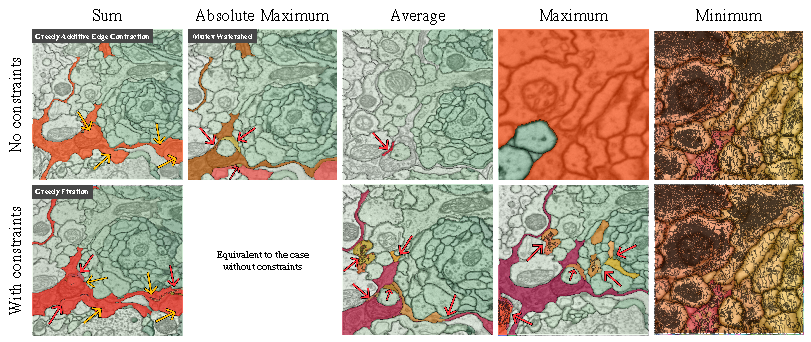
\includegraphics[width=\textwidth]{./figs/comparison_new.pdf} % left bottom right top
\caption{Failure cases of \algname{} with different linkage criteria highlighted on some difficult parts of the CREMI Challenge data. Only the \emph{wrongly} segmented regions are highlighted in different warm colors. Note that the data is 3D, hence the same color could be assigned to parts of segments that appear disconnected in 2D.  Red arrows point to wrongly split regions. Yellow arrows point out merge errors. The \emph{Average} linkage without cannot-link constraints returned the best segmentation.
\label{fig:cremi_comparison}}
\end{figure*}



\begin{table*}[t]
    \centering
    % \scriptsize
    \tiny
    \begin{subtable}[t!]{\textwidth}\centering
        \begin{tabular}{l  c  c  c  c  c c c c c c c c c}
        \toprule
        Dataset & Graph-Type & $\#I$ & $|V|$ & $\bar{\text{deg}}(v)$ & GT & GAEC & MWS & HC-AvgL & HC-SingleL & HC-CompleteL & Constr-SumL & Constr-AvgL & Constr-SingleL \\ \midrule
        \emph{Image Seg.} & \emph{rag} & 100 & 156-3764 &   & \HollowBox\\
        \emph{Knott-3D (150-300-450)} & \emph{rag-3D} & 24 & 572-17k &  & \HollowBox\\
        % \emph{Knott-3D-300} & \emph{rag-3D} & 8& & & \HollowBox\\
        % \emph{Knott-3D-450}& \emph{rag-3D} & 8 & & & \HollowBox\\  
        \emph{CREMI-OurUNet} & \emph{rag-3D} & 3&  & & \CrossedBox\\ 
        \emph{Fruit-Fly Level 1-4} & \emph{rag-3D} & 4& 5m-11m &  & \HollowBox\\
        \emph{Fruit-Fly Level Global} & \emph{rag-3D} & 1& 90m &  & \HollowBox\\ \midrule
                \emph{CREMI-pixGrid-OurUNet} & \emph{gridGraph} & 12& $\sim$30m & 4 & \CrossedBox\\
        % \emph{(CREMI-pixGrid-LSIMasksUNet)} & \emph{gridGraph} & 1 & & 4 & \CrossedBox\\
        \emph{(CityScapesValidation-pixGrid)} & \emph{gridGraph} &  &  & & \CrossedBox\\\midrule
        % \emph{CREMI-test....}\\\midrule
        \emph{Stochastic Block Model (synthetic)} & \emph{non-planar} &-&- & - & \CrossedBox \\
        \emph{Mod. Clustering} & \emph{complete} & 6& 34-115 & 33-114 & \HollowBox\\ 
        \emph{(epinions and slashdot?)} & \emph{dense?} &  & & & \HollowBox\\ 
        
        


            
        \end{tabular}
    \end{subtable} 
    \caption{List of used datasets and MC objectives achieved by different algorithms} 
    \label{tab:datasets_and_energies}
\end{table*}


% \begin{table}[t]
%     \centering
%     % \scriptsize
%     \tiny
%     \begin{subtable}[t!]{0.5\textwidth}\centering
%         \begin{tabular}{l  c  c  c  c  c}
%         \toprule
%         Dataset & HC-Avg & GAEC & MWS & Constr-Avg & Constr-Sum \\ \midrule
%         \emph{Image Seg.} \\
%         \emph{Knott-3D-150} \\
%         \emph{Knott-3D-300} \\
%         \emph{Knott-3D-450} \\  
%         \emph{Mod. Clustering} \\
%         \emph{Fruit-Fly Level 1-4} \\
%         \emph{Fruit-Fly Level Global} \\
%         \emph{(Epinions?)} \\
        


            
%         \end{tabular}
%     \end{subtable} 
%     \caption{} 
%     \label{tab:all_results}
% \end{table}


% !TEX root = ../agglo_clust_review.tex

\section{Estimating edge weights}
\begin{itemize}
\item Define predictions of the classifier (pseudo probabilities) for edge weights
\item Define possible mappings to signed costs
\item Make comment about which version defines nested segmentations and which does not give hirarchical solutions

\end{itemize}


\section{Experiments}
% !TEX root = ../agglo_clust_review.tex



\section{Experiments on neuron segmentation}\label{sec:neuro_segm_exp}

We first evaluate and compare the agglomerative clustering algorithms described in the generalized framework on the task of neuron segmentation in electron microscopy (EM) image volumes. This application is of key interest in connectomics, a field of neuro-science with the goal of reconstructing neural wiring diagrams spanning complete central nervous systems. Currently, only proof-reading or manual tracing yields sufficient accuracy for correct circuit reconstruction \cite{schlegel2017learning}, thus further progress is required in automated reconstruction methods.
%First, we present how we predicted signed edge weights with a CNN. Then we introduce the CREMI challenge and our tested methods in Sec. \ref{sec:cremi_challenge} and finally we present our results in Sec. \ref{sec:results}.

% \subsection{Experimental setup: pixel grid-graph with long-range connections} \label{sec:grid_graph}
EM segmentation is commonly performed by first predicting 
% which pixels belong to a cell membrane using a CNN. As described in Sec. \ref{sec:related_work}, different postprocessing methods are then used to obtain a segmentation. The CNN can either be trained to predict 
boundary pixels \cite{beier2017multicut,ciresan2012deep} or undirected affinities \cite{wolf2018mutex,lee2017superhuman,funke2018large}, which represent how likely it is for a pair of pixels to belong to the same neuron segment. 
The affinities do not have to be limited to direct neighboring pixels
Thus, similarly to \cite{lee2017superhuman}, we train a CNN to predict both short- and long-range affinities
and use them as edge weights of a 3D grid graph, where each node represents a pixel/voxel of the volume image. 
% In our experiments, we divided the set of edges $E$ in $E_{\mathrm{direct}}$ connecting direct neighboring voxels and $E_{\mathrm{long}}$. 
% See Appendix \ref{sec:training_details} for more details on the chosen neighborhood structure.
% , data augmentation and the training with L1 loss of the used 3D U-Net architecture \cite{ronneberger2015u,cciccek20163d}.
% We evaluate how beneficial long-range connections are by adding 
% The output layer of the CNN will then have $m_{\mathrm{direct}}+m_{\mathrm{long}}$ channels, where $m_{\mathrm{direct}}=6$ represents the direct neighbors in 3D and $m_{\mathrm{long}}$ is the number of long-range ones. 
% The output of the CNN can be represented as a weighted 3D grid graph, such that each node represents a pixel/voxel of the volume image. Each node is connected to its neighbors by $m_{\mathrm{direct}}$ edges ($E_{\mathrm{direct}}$) and $m_{\mathrm{long}}$ long-range ones ($E_{\mathrm{long}}$).
% In our experiments we evaluate how beneficial long-range connections are for the final segmentation and we add them to the graph with a given probability $p_{\mathrm{long}}$ (if $p_{\mathrm{long}}=0$, then $E_{\mathrm{long}}=\emptyset$).
% We note that the post-processing presented in \cite{lee2017superhuman} did not use any predicted long-range connection, whereas \cite{wolf2018mutex} introduced them with strides of 2 in the XY-plane.


% !TEX root = ../agglo_clust_review.tex


\begin{figure}
        \centering
\begin{minipage}[T]{0.48\textwidth}
% \begin{table}
    \centering
    \scriptsize
    % \begin{subtable}[t!]{0.5\textwidth}\centering
        \begin{tabular}{l|l|c}
        % \toprule
        % & \multicolumn{2}{c}{\thead{Add Cannot-Link Constraints:}} \\
         % & \multicolumn{1}{c}{\thead{\textsc{No}}} & \multicolumn{1}{c}{\thead{\textsc{Yes}}} \\ \midrule
         & \algname{} Linkage & \makecell{Arand-Score}  \\ \midrule \midrule
         % & \multicolumn{1}{c}{\thead{$\beta$}}  & \thead{AP} & \multicolumn{1}{c}{\thead{$\beta$}} & \thead{AP} \\ \midrule\midrule
\textbf{\algname{}} & \textbf{Average}& \textbf{0.936 $\pm$ 0.004}  \\
Greedy Fixation \cite{levinkov2017comparative} & Sum + Constr. & 0.906 $\pm$ 0.022 \\
DTWS + LMC (LR)& -& 0.903 $\pm$ 0.016 \\
DTWS + MC (LR)& -& 0.903 $\pm$ 0.017 \\
% DTWS + avgHC &-& \\
DTWS + MC (SR)& -& 0.900 $\pm$ 0.019 \\
DTWS + LMC (SR)& -& 0.898 $\pm$ 0.017 \\
Mutex Watershed \cite{wolf2018mutex} & Abs. Max.  & 0.897 $\pm$ 0.012 \\
GAEC \cite{keuper2015efficient} & Sum & 0.872 $\pm$ 0.028 \\
THRESH &-& 0.221  $\pm$ 0.067 \\ 
DTWS  & -& 0.010 $\pm$ 0.003\\
        \end{tabular}
    \captionof{table}{Arand-Scores and VI-Scores on CREMI challenge training data}
    \label{tab:results_cremi_train}
\end{minipage}\hfill
\begin{minipage}[T]{0.48\textwidth}
    \centering
    \scriptsize
        \begin{tabular}{l|c|c}
         & \makecell{CREMI \\Score} & \makecell{Arand\\Score} \\ \midrule
Our UNet + DTWS + LMC &  \textbf{0.221} & \textbf{0.108}\\
PNI-UNet & 0.228 & 0.116 \\
Our UNet + \algname{} Avg-Linkage & 0.244 & 0.130 \\
MALA-UNet + MC \cite{funke2018large} & 0.276 & 0.132 \\
CRUNet \cite{zeng2017deepem3d} & 0.566 & 0.229 \\
LFC \cite{parag2017anisotropic} & 0.616 & \\
        \end{tabular}
    \captionof{table}{\UPDATE{TBD:} Scores on test data}
    \label{tab:results_cremi_test}
\end{minipage}
\end{figure}

\subsection{CREMI Challenge} \label{sec:cremi_challenge}
We evaluate the algorithms in our framework on the competitive CREMI 2016 EM Segmentation Challenge \cite{cremiChallenge} that is currently the neuron segmentation challenge with the largest amount of training data available. The dataset comes from a serial section EM of \emph{Drosophila} fruit-fly tissue and consists of 6 volumes of 1250x1250x125 voxels at resolution 4x4x40nm, three of which present publicly available training ground truth. The results submitted to the leaderboard are evaluated using the CREMI score\footnote{\url{https://cremi.org/leaderboard/}}, based on the Adapted Rand-Score (Rand-Score) and the Variation of Information Score\cite{arganda2015crowdsourcing}. The data is highly anisotropic and contains artifacts like missing sections, staining precipitations and support film folds. 

\textbf{Training details}
To alleviate difficulties stemming from misalignment, we use a version of the data that was elastically realigned by the challenge organizers with the method of \cite{saalfeld2012elastic}.
We train a 3D U-Net \cite{ronneberger2015u, cciccek20163d} using the same architecture as \cite{funke2018large} and predict long-and-short range affinities 
as described in \cite{lee2017superhuman}. In addition to the standard data augmentation techniques of random rotations, random flips and  elastic deformations, we simulate data artifacts.
In more detail, we randomly zero-out slices, decrease the contrast of slices, simulate tears, introduce alignment jitter and paste artifacts extracted from the training data. Both \cite{funke2018large} and \cite{lee2017superhuman} have shown
that these kinds of augmentations can help to alleviate issues caused by EM-imaging artifacts.
We use L2 loss and Adam optimizer to train the network.
%\UPDATE{We pre-aligned the training and test data with an elastic alignment method \cite{saalfeld2012elastic}. We further simulated low contrast sections... and missing sections by setting their intensity value to zero... We used 3D U-Net architecture \cite{ronneberger2015u,cciccek20163d} trained with L1 loss (Adam optimizer with learning rate...).} 

\textbf{Additional methods tested }  We compare the performances of the algorithms in our framework with other basic and state-of-the-art post-processing methods. To ensure a fair comparison, we test all methods on the same predictions of our CNN model. As baseline methods, we consider a simple thresholding (THRESH) and a watershed algorithm seeded at the maxima of a boundary distance transform (WSDT). For these baselines, affinities are converted to a boundary map \UPDATE{by taking a weighted average over short- and long-range edge connections}. Other state-of-the-art multi-step-pipelines for neuron-segmentation first find 2D superpixels using WSDT and then apply a graph partitioning algorithm: in our comparison, we include one pipeline using agglomerative HC with average linkage (avgHC) and one using an approximation of the Lifted Multicut Problem (LMC) \cite{beier2016efficient}.



% !TEX root = ../agglo_clust_review.tex
% 

\begin{figure}
\centering
        \begin{subfigure}[t]{0.48 \textwidth}
        \centering
        \includegraphics[width=0.98\textwidth,trim=0.35in 0.35in 0.35in 0.35in,clip]{./figs/merge_noise.pdf}

        \caption{Merge-biased opensimplex noise} \label{fig:thresh}
    \end{subfigure}%
    \begin{subfigure}[t]{0.48 \textwidth}
        \centering
        \includegraphics[width=0.98\textwidth,trim=0.29in 0.31in 0.31in 0.31in,clip]{./figs/split_noise.pdf}
        \caption{Split-biased opensimplex noise} \label{fig:ws}
    \end{subfigure}


\caption{Plot illustrating Adapted RAND scores achieved by UGACA and different update rules when noise is added to the edge weights... Solid lines represent median values, whereas values between the 25th and the 75th percentile are shown in shade areas.    \TODO{Label which uses only local-neighbors and which uses long-range connections}}\label{fig:noise_plots}
\end{figure}

% \begin{minipage}[b]{0.48\textwidth}
% % \begin{figure}
%         % \begin{subfigure}[t]{0.48 \textwidth}
%         \centering
%         \includegraphics[width=0.98\textwidth,trim=0.35in 0.35in 0.35in 0.35in,clip]{./figs/merge_noise.pdf}

%         \captionof{subfigure}{Merge-biased opensimplex noise} \label{fig:thresh}
%     \end{minipage}\hfil
% \begin{minipage}[b]{0.48\textwidth}
%     % \end{subfigure}%
%     % \begin{subfigure}[t]{0.48 \textwidth}
%         \centering
%         \includegraphics[width=0.98\textwidth,trim=0.29in 0.31in 0.31in 0.31in,clip]{./figs/split_noise.pdf}
%         \captionof{subfigure}{Split-biased opensimplex noise} \label{fig:ws}
%     % \end{subfigure}
% \captionof{figure}{Plot illustrating Adapted RAND scores achieved by UGACA and different update rules when noise is added to the edge weights... Solid lines represent median values, whereas values between the 25th and the 75th percentile are shown in shade areas.    \TODO{Label which uses only local-neighbors and which uses long-range connections}}\label{fig:noise_plots}
% % \end{figure}



\subsection{Testing the robustness of the algorithms}
 In this section we will quantitatively test the robustness of UGACA by adding noise to the edge weights of the graph and see how different choices of update rules compare.
 Among the update rules listed in Table \ref{tab:linkage-criteria}, we will only focus on \emph{sum}, \emph{arithmetic mean} and \emph{absolute maximum}, since they achieved the best scores in the results presented in Sec. \ref{sec:exp_first_comparison}. %Before to present the results shown in Fig. \ref{fig:noise_plots}, we will first introduce the type of noise that was added to the edge weights.

 In the set of experiments presented in this article, edge weights are estimated \UPDATE{by using a CNN that predicts how likely two neighboring pixels are to be part of the same cluster}. Fig. \hyperref[fig:noisy_affs]{\ref*{fig:noisy_affs}a} illustrates the predictions of the CNN on the CREMI dataset for neuron segmentation. We would now like to make these predictions worse by introducing  artifacts, \UPDATE{e.g. partially deleted or added boundaries between neurons in the image}. In the field of image processing there are several ways of adding noise to an image, among which the most common are Gaussian noise or Poisson shot noise. By using these methods, the noise value of each pixel is independent of noise values of neighboring pixels, thus they are not a good choice for our application since the pixelwise predictions of a CNN are usually spatially correlated. 

 We then decided to use Perlin noise\footnote{In our experiments, we used opensimplex noise, that is a more recent open-source version of Perlin noise (\UPDATE{REF or link?})}, one of the most common gradient noises used in procedural pattern generation. This type of noise generates spatial random patterns that are locally smooth but have large and diverse variations on bigger scales. It generates values $n(x)\in[0,1]$ that were mapped to $[-\infty, \infty]$ with the Logit function, $N(x)=\mathrm{Logit}(n(x))$, and then combined with the original CNN predictions $F(x)=\mathrm{Logit}(p(x))$ in the two different following ways:
\begin{equation}
% \tilde{F}(x;\theta)=\begin{cases}
% F(x;\theta)+\mathcal{K}\cdot\max\left(N(x),0\right) & \text{if merge-biased}\\
% F(x;\theta)+\mathcal{K}\cdot\min\left(N(x),0\right) & \text{if split-biased}
% \end{cases}
\tilde{F}_{\pm}(x;\mathcal{K})=F(x)\pm\big|\mathcal{K}\cdot\max\left(\pm N(x),0\right)\big|,
\end{equation}
In this equation, $\mathcal{K}\in \mathbb{R}^+$ is a positive factor representing the amount of added noise; $\tilde{F}_{+}(x;\mathcal{K})$ represents a merge-biased modified version of the CNN predictions $F(x)$, such that the probability for two pixels to be in the same cluster is increased only if $N(x)>0$ (see Fig. \hyperref[fig:noisy_affs]{\ref*{fig:noisy_affs}b}); on the other hand, $\tilde{F}_{-}(x;\mathcal{K})$ represents a split-biased prediction with decreased probabilities only if $N(x)<0$ (Fig. \hyperref[fig:noisy_affs]{\ref*{fig:noisy_affs}c}). In the Supplementary material we provide a detailed description of the parameters used for the noise generation.

With this strategy, we randomly perturbed the CNN predictions and the edge weights only in some parts of the image. The plots in Fig. \ref{fig:noise_plots} represent the scores achieved by UGACA with different update rules depending on the amount of noise $\mathcal{K}$ added to the edge weights. 
\begin{itemize}
\item The experiments show that running UGACA on a grid graph with long-range connections always lead to better segmentations/clusterings \TODO{require def. of long range graph and long-range probability}
\item The most robust version of update rule proved to be the arithmetic mean, that achieves similar scores even with significantly noisy edge weights.
\item The \emph{absolute maximum} update rule proposed by \cite{wolf2018mutex} provides an efficient and fast option, but it completely fails when too much noise is added.
\item The \emph{sum} update rule version was the slowest option tested, but it was not as robust as the \emph{mean} version, probably due to its tendency to grow one cluster at the time (see Sec. \ref{sec:exp_first_comparison}). Comment about MC energy (plots in Suppl. Material?)
\item On the other hand, UGACA with mean update rule and cannot-link constraints never achieves good overall scores, as we have already shown in Sec. \ref{sec:exp_first_comparison} and \UPDATE{Figure...?}, because \UPDATE{it tends to introduce too many false splits}. 
%Nevertheless, these additional experiments show that it provides an \UPDATE{almost true over-segmentation of the ground truth segmentation even with strongly merge-biased predictions}.
\end{itemize}

\begin{minipage}[T!]{\textwidth}
        \centering
        \begin{minipage}{0.45\textwidth}
\centering

        \includegraphics[width=0.85\textwidth,trim=0.1in 0.0in 0.05in 0.0in,clip]{figs/noisy_affs_comparison.png}
   
    \captionof{figure}{The two figures represent the predictions of the CNN on the CREMI dataset (\UPDATE{REF}) a) without added noise, b) with the addition of the merge-biased noise defined in Eq. \ref{eq:opensimplex_noise_def} and c) with split-biased noise. The color of each pixel represents how probable it is for it to be in the same cluster with its neighboring pixel on the right (red: same cluster; blue: different ones). 
    %Adding merge-biased noise tends to create holes in the boundaries; split-biased noise add non-existing boundaries 
    \TODO{Add colorbar? Adapt to noise defs}}
    \label{fig:noisy_affs}
    \end{minipage}\hspace{0.04\textwidth}
\begin{minipage}{0.48\textwidth}
% \begin{table}
    \centering
    % \begin{subtable}[t!]{0.5\textwidth}\centering
        \begin{tabular}{l M{0.25\textwidth} M{0.25\textwidth}}
        \toprule
        & \multicolumn{2}{c}{\thead{Add Cannot-Link Constraints:}} \\
        Update rule: & \multicolumn{1}{c}{\thead{\textsc{No}}} & \multicolumn{1}{c}{\thead{\textsc{Yes}}} \\ \midrule
         % & \multicolumn{1}{c}{\thead{$\beta$}}  & \thead{AP} & \multicolumn{1}{c}{\thead{$\beta$}} & \thead{AP} \\ \midrule\midrule
\textbf{Mean}& \textbf{0.343}  & 0.339  \\
GMIS \cite{liu2018affinity} & 0.341 & -  \\
Max &   0.243  &   0.325  \\
Abs. Max. \cite{wolf2018mutex}  & -  & 0.321 \\
Sum \cite{levinkov2017comparative} & 0.313  & 0.319  \\
Min &  0.000    & 0.000  \\
        \end{tabular}
        % \caption{Linkage criteria}
    % \end{subtable} 
    \captionof{table}{AP scores on the cityscapes validation set for UGACA and different types of update rules. \TODO{PROBLEM: all apart from GMIS uses finetuned affinities} }
    \label{tab:results_cityscapes}
\end{minipage}
\end{minipage}

% \begin{equation}
% \begin{gathered}
% \tilde{p}_{\pm}(x;\theta)=\sigma(\tilde{F}_{\pm}(x;\theta))\quad \text{where}\\
% % \tilde{F}(x;\theta)=\begin{cases}
% % F(x;\theta)+\mathcal{K}\cdot\max\left(N(x),0\right) & \text{if merge-biased}\\
% % F(x;\theta)+\mathcal{K}\cdot\min\left(N(x),0\right) & \text{if split-biased}
% % \end{cases}
% \tilde{F}_{\pm}(x;\theta)=F(x;\theta)\pm\left|\mathcal{K}\cdot\max\left(\pm N(x),0\right)\right|
% \end{gathered}
% \end{equation}

% !TEX root = ../agglo_clust_review.tex
\section{Experiments on CityScapes}\label{sec:cityscapes_exp}
We also evaluate the performances of \algname{} on the CityScapes dataset \cite{cordts2016cityscapes}, which consists of 5000 street-scene images: 2975 for training, 500 for validation and 1525 for testing.
% recorded by car-mounted cameras with resolution 1024$\times$2048: 2975 images for training, 500 for validation and 1525 for testing. Objects with instance-level annotations belong to the following classes: person, rider, car, truck, bus, train, motorcycle, bicycle. 
For our experiments, we used the state-of-the-art proposal-free pipeline proposed in GMIS \cite{liu2018affinity} that achieved superior performances compared to other proposal-based methods like Mark R-CNN and employs a similar model to the one applied by us on neuron-segmentation.
Their trained model was made publicly available, so we simply replaced their final graph-merging algorithm (MultiStepHAC) with \algname{}. See Appendix \ref{sec:appendix_cityscapes} for more details on how we fine-tuned their instance branch model by using a \emph{S\o resen-Dice} loss similarly to \cite{wolf2018mutex} and obtained in this way sharper affinity-predictions.

Results are summarized in Table \ref{tab:results_cityscapes_val} and confirm our findings on neuron-segmentation: \algname{} with average linkage achieves the best scores, whereas other linkage tend to introduce more false region-splits, like \emph{Abs. Max.}, or false region-merge, like \emph{Sum}. In Appendix, Table \ref{tab:extended_results_cityscapes_val} includes all other tested linkage. MultiStepHAC requires the user to tune several threshold parameters and it was probably tailored to the original affinities predicted by \cite{liu2018affinity}, so it did not generalize well to our fine-tuned model and it achieved lower scores compared to the original AP value of 34.1 reported in \cite{liu2018affinity}.  


\begin{figure}[t]
\centering
\begin{minipage}[T]{0.59\textwidth}
    \centering
    \footnotesize
        \begin{tabular}{l|l|cc}
           & Agglomeration  &  \multicolumn{2}{c}{Use constraints:} \\
          Pipeline & method & \textsc{No} & \textsc{Yes} \\ \midrule
DWT \cite{bai2017deep} & - & 21.2 & - \\
SGN \cite{liu2017sgn} & - & 29.2 & - \\
Mask RCNN \cite{he2017mask} & - & 31.5 & - \\ \hline
 & \textbf{\algname{} Average}& \textbf{34.3}  & 33.9  \\
\multirow{2}{*}{GMIS \cite{liu2018affinity}} & MultiStepHAC \cite{liu2018affinity} & 33.0 & -  \\
 % & \algname{} Max &   24.3  &   32.5  \\
 & \algname{} Abs. Max. \cite{wolf2018mutex}  & 32.1 & 32.1 \\
 & \algname{} Sum \cite{keuper2015efficient,levinkov2017comparative} & 31.3  & 31.9  \\
 % & \algname{} Min &  0    & 0  \\
        \end{tabular}
    \captionof{table}{Average Precision (AP) scores on the cityscapes validation set achieved by the tested pipelines}
    \label{tab:results_cityscapes_val}
\end{minipage}\hfill
\begin{minipage}[T]{0.37\textwidth}
    \centering
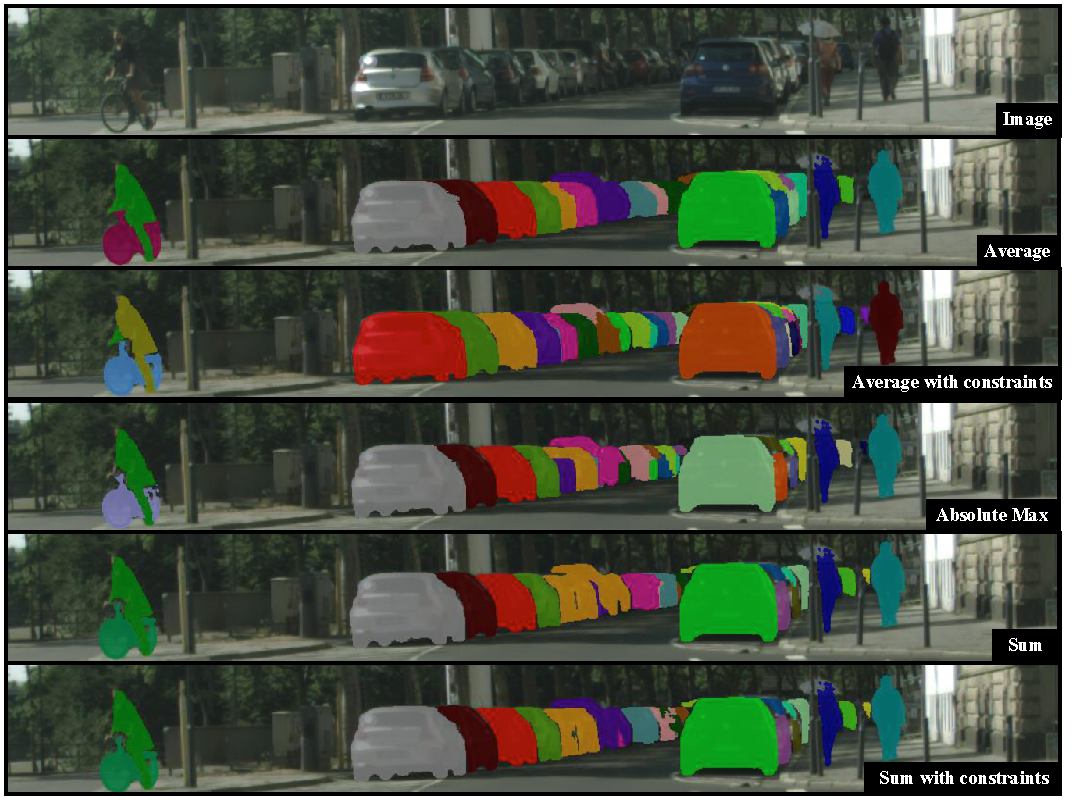
\includegraphics[width=\textwidth]{./figs/cityscapes_compare_2.pdf} % left bottom right top
\end{minipage}
\end{figure}

% !TEX root = ../agglo_clust_review.tex
\subsection{Results on CREMI challenge}



% !TEX root = ../agglo_clust_review.tex
\section{Conclusion}
We presented both a theoretical and experimental contribution: ; why average is so cool?

We presented a generalized framework and showed how one of the new algorithms included in it, \algname{} with average linkage, represent a simple agglomerative method that does not require the user to tune parameters or generate superpixels and showed extremely competitive performances in biological images, even on the challenging and competitive task of neuron segmentation. (good-quality superpixels are strongly dataset-dependent)
Compared to previously proposed agglomerative clustering methods for signed graphs, it proved to be the one making best use of the long-range predictions of the CNN; the fact that average is superior to abs max is not surprising, given the literature about HAC with single and average linkage (due to the greediness of the maximum linkage); and enforcing cannot-link constraints, we have also seen that introducing too many long-range mainly repulsive predictions can cause strong over-clustering; tendency to under-clustering of the sum linkage can be explained with the chain-reaction effect and its tendency to grow one cluster at the time that does not allow to build good statistics between adjacent clusters. This is partially fixed by constraints, but not really...


{\small
\bibliographystyle{abbrv}
\bibliography{agglo_clust}
}
% !TEX root = ../agglo_clust_review.tex

\begin{figure}
        \centering
\begin{minipage}{0.45\textwidth}
\centering
        \includegraphics[width=0.85\textwidth,trim=0.1in 0.0in 0.05in 0.0in,clip]{figs/noisy_affs_comparison.png}
   
    \captionof{figure}{The two figures represent the CNN predictions on a slice of the neuron segmentation CREMI challenge \cite{cremiChallenge} with and without additional noise. Blue pixels represent boundary evidence. Image a) shows the original CNN predictions, b) the merge-biased version $\tilde{F}_{+}$ and c) the split-biased version $\tilde{F}_{-}$ (see definition \ref{eq:noise_biased_predictions}). 
    %The color of each pixel represents how probable it is for it to be in the same cluster with its neighboring pixel on the right (red: same cluster; blue: different ones). 
    %Adding merge-biased noise tends to create holes in the boundaries; split-biased noise add non-existing boundaries 
    }
    \label{fig:noisy_affs}
    \end{minipage}\hfill
\begin{minipage}{0.49\textwidth}
\centering
        % \includegraphics[width=\textwidth,trim=0.1in 0.4in 0.2in 0.2in,clip]{./figs/edge_contraction.png} % left bottom right top
        \includegraphics[width=\textwidth]{./figs/edge_contraction.pdf} % left bottom right top
\captionof{figure}{ 
{\small Example of edge contraction. First row: original graph $\mathcal{G}$; clustering $\Pi$ (gray shaded areas) with dashed edges on cut; cannot-link constraints (violet bars). Second row: contracted graph $\tilde{\mathcal{G}}_\Pi$. In step ii), edge $e_{uv}$ is contracted and node $v$ deleted from $\tilde{\mathcal{G}}_\Pi$. In step iii), double edges $e_{tu}$ and $e_{tv}$ resulting from edge contraction are replaced by single edge with updated interaction $f(\tilde{\cost}(e_{tu}), \tilde{\cost}(e_{tv}))$, see definitions in Tab.~\ref{tab:linkage-criteria}. }
\label{fig:edge_contraction_and_contr_graph}  }
    \end{minipage}
\end{figure}


\section{Supplementary Material}
During the agglomerative process, the interaction between adjacent clusters has to be properly updated and recomputed.  % given by the linkage criterion defined in Sec. \ref{sec:notation} and
Given a graph $\mathcal{G}(V,E,\cost)$ and a clustering $\Pi$, we define the \emph{contracted graph} $\tilde{\mathcal{G}}_\Pi(\tilde{V}, \tilde{E}, \tilde{\cost})$, with $\tilde{V} \subseteq V$ such that node $u\in \tilde{V}$ represents the associated cluster $S_u \in \Pi$. Edges in $\tilde{E}$ are defined by adjacency-relationships between clusters and edge weights $\tilde{\cost}_{uv}$ represent inter-cluster interactions $\interact(S_u,S_v)$. 



\paragraph{Update rules} During the agglomerative process, the interaction between adjacent clusters has to be properly updated and recomputed.  % given by the linkage criterion defined in Sec. \ref{sec:notation} and
An efficient way of implementing these updates can be achieved by representing the agglomeration as a sequence of \emph{edge contractions} in the graph. Given a graph $\mathcal{G}(V,E,\cost)$ and a clustering $\Pi$, we define the associated \emph{contracted graph} $\tilde{\mathcal{G}}_\Pi(\tilde{V}, \tilde{E}, \tilde{\cost})$, such that $\tilde{V} \subseteq V$ and each node $u\in \tilde{V}$ represents the cluster $S_u \in \Pi$ including $u\in V$. Edges in $\tilde{E}$ represent adjacency-relationships between clusters and the signed edge weights $\tilde{\cost}_e$ are given by inter-cluster interactions $\tilde{\cost}(e_{uv})=\interact_{S_u,S_v}$. 
For the linkage criteria tested in this work, when two clusters $S_u$ and $S_v$ are merged, the interactions between the new cluster $S_u \cup S_v$ and each of its neighbors depend only on the previous interactions involving $S_u$ and $S_v$. Thus, we can easily recompute these interactions by using a simple \emph{update rule} $f$ that does not involve any loop over the edges of the original graph $\mathcal{G}$. As an example, given the single-linkage criterion defined in Eq. \ref{eq:max_linkage}, the interaction between $S_u \cup S_v$ and one of its neighbors $S_t$ is simply given by:
\begin{equation}
  \interact_{S_u \cup S_v,S_t} = f( \interact_{S_u,S_t}, \interact_{S_v,S_t}) = f(\tilde{\cost}(e_{ut}), \tilde{\cost}(e_{vt})) = \max \{ \tilde{\cost}(e_{ut}), \tilde{\cost}(e_{vt}) \}
\end{equation}
All the update rules tested in this article are listed in Table \ref{tab:linkage-criteria}.

% \UPDATE{Every time a pair of clusters is merged, the contracted graph is updated by performing an edge contraction and merging the associated nodes. The only interactions that then need to be updated are those between nodes that after the edge contraction happen to be connected by double edges (see Fig. \ref{fig:edge_contraction_and_contr_graph}, step b). For basic linkage criteria, e.g. \emph{max} or \emph{min}, the new interaction can be formulated in terms of an \emph{update rule} $f$ depending only on the these updates can be computed with an update rule $f$ that depends only on the interactions at the previous step }
% As a result, the merged node could be linked to some of its neighbors by double edges . , representing the fact that their interaction should be updated. This update can be easily achieved by using an \emph{update rule} depending only on the weights of the double edges. 
% \TODO{such a mess...} ...without the need of running a loop over the edges of the original graph.
% \UPDATE{In this way we do not need to recompute the interaction by using the linkage criterion over all the edges of the original graph, that would be computationally expensive.}
\textbf{The proposed edge contraction algorithm } Algorithm \ref{main_alg} then proceeds as follows, similarly to the one presented in \cite{levinkov2017comparative}. It starts with each node assigned to its own cluster and sorts all edges $e\in E$ in a priority queue (PQ) by their absolute weight $|\cost_e|=|w_e^+ - w_e^-|$ in descending order, so that the most attractive and the most repulsive interactions are processed first. It then iteratively pops one edge $e_{uv}$ from PQ and, depending on the priority $\tilde{\cost}$, does the following: in case of attractive interaction $\tilde{\cost}>0$, provided that $e_{uv}$ was not flagged as a cannot-link constraint, then merge the connected clusters, perform an edge contraction of $e_{uv}$ in $\tilde{\mathcal{G}}_\Pi$ and update the priorities of new double edges as explained in Fig. \ref{fig:edge_contraction_and_contr_graph}. 
% For every new pair of double edges in $\tilde{\mathcal{G}}_\Pi$, update their priorities according to one of the update rules listed in Table \ref{tab:linkage-criteria} together with their cannot-link relationships. 
If, on the other hand, the interaction is repulsive ($\tilde{\cost}\leq 0$) and the option \texttt{addCannotLink} of Alg. \ref{main_alg} is \texttt{True}, then the edge $e_{uv}$ is flagged as cannot-link constraint.
In the Supplementary material we comment on the algorithm computational complexity (Sec. \ref{sec:complexity}).



\begin{itemize}
\item Equivalence Mutex Watershed and Greedy Edge Contraction
\item Complexity: plain agglo., addition of the cannot-link constraints and then comment about efficient implementation of MWS and of single-linkage (what about single linkage+CLC...?)
\item Noise: also mention details about plots (fix some long-range edges, fix noise seed and vary K)
\item exp. setup details: enforcing local merges, MWS distinguish between repulsive-long, post-processing of small segments, loss, architecture, training parameters, offset patterns
\item 

\end{itemize}

\subsection{Noise exps}
 % In this section we evaluate the robustness of \algname{} with different linkage criteria by adding noise to the edge weights.
  %Before to present the results shown in Fig. \ref{fig:noise_plots}, we will first introduce the type of noise that was added to the edge weights.
% In the set of experiments presented in this article, edge weights are estimated \UPDATE{by using a CNN that predicts how likely two neighboring pixels are to be part of the same cluster}. 
Fig. \hyperref[fig:noisy_affs]{\ref*{fig:noisy_affs}a} shows an example of uncertain CNN predictions on a slice of the neuron segmentation dataset. We now present a way of modifying the CNN output to introduce additional artifacts like a missing or false boundary evidence. 

In the field of image processing there are several ways of adding noise to an image, among which the most common are Gaussian noise or Poisson shot noise. 
In these cases, the noise of one pixel does not correlate with its neighboring noise values. On the other hand, predictions of a CNN are known to be spatially correlated. 
Thus, we used Perlin noise\footnote{In our experiments, we used an open-source version of simplex noise \cite{perlin2001noise}, which is an improved open-source version of Perlin noise \cite{perlin1985image}}, one of the most common gradient noises used in procedural pattern generation. This type of noise $n(x)\in[0,1]$ generates spatial random patterns that are locally smooth but have large and diverse variations on bigger scales. We then combined it with the CNN predictions $p(x)$ in the two following ways: 
\begin{equation}\label{eq:noise_biased_predictions}
% \tilde{F}(x;\theta)=\begin{cases}
% F(x;\theta)+\mathcal{K}\cdot\max\left(N(x),0\right) & \text{if merge-biased}\\
% F(x;\theta)+\mathcal{K}\cdot\min\left(N(x),0\right) & \text{if split-biased}
% \end{cases}
\tilde{F}_{\pm}(x;\mathcal{K})=F(x)\pm\big|\mathcal{K}\cdot\max\left(\pm N(x),0\right)\big|,
\end{equation}
where  $N(x)=\mathrm{Logit}[n(x)]$; $F(x)=\mathrm{Logit}[p(x)]$ and $\mathcal{K}\in \mathbb{R}^+$ is a positive factor representing the amount of added noise. $\tilde{F}_{+}(x;\mathcal{K})$ represents then a merge-biased prediction, such that the probability for two pixels to be in the same cluster is increased only if $N(x)>0$ (see Fig. \hyperref[fig:noisy_affs]{\ref*{fig:noisy_affs}b}), whereas $\tilde{F}_{-}(x;\mathcal{K})$ is a split-biased prediction with decreased probabilities when $N(x)<0$ (Fig. \hyperref[fig:noisy_affs]{\ref*{fig:noisy_affs}c}). In the Supplementary material (Sec. \ref{sec:details_perlin}) we provide a more detailed description of the parameters used for the noise generation.


\subsection{Cityscapes exps}
Mention the main trick in the loss: ignore background pixels (so focus on boundaries). Same mapping defined in \ref{eq:mappings}


\begin{table*}
    \centering
    \begin{subtable}[t!]{0.98\textwidth}\centering
        \begin{tabular}{c| c | c| c | c | c | c | c}
Update rule & \makecell{Use Cannot-Link\\Constraints} & Log-costs & \makecell{Multicut objective} & Runtime (s) & ARAND & VI-merge & VI-split\\ \midrule\midrule
% \textbf{mean} & False & \textbf{-102739991} & {\color{Orange} 3797 } & {\color{ForestGreen} \textbf{0.0708} } & {\color{ForestGreen} 0.286 } & {\color{ForestGreen} 0.428 } \\
% % mean & False & -102730208 & {\color{Orange} 2562 } & {\color{ForestGreen} 0.0715 } & {\color{ForestGreen} 0.292 } & {\color{ForestGreen} 0.423 } \\
% MutexWatershed & False & -102313957 & {\color{ForestGreen} 830 } & {\color{ForestGreen} 0.0754 } & {\color{ForestGreen} 0.291 } & {\color{Orange} 0.471 } \\
% sum & False & -101846418 & {\color{Red} 12681 } & {\color{Orange} 0.1623 } & {\color{Orange} 0.427 } & {\color{ForestGreen} 0.427 } \\
% % sum & False & -101732952 & {\color{Red} 12287 } & {\color{Orange} 0.1624 } & {\color{Orange} 0.436 } & {\color{ForestGreen} 0.390 } \\
% sum & True & -101487448 & {\color{Red} 8497 } & {\color{Orange} 0.1626 } & {\color{Orange} 0.428 } & {\color{ForestGreen} 0.414 } \\
% % sum & True & -100745943 & {\color{Red} 13361 } & {\color{Orange} 0.1574 } & {\color{Orange} 0.410 } & {\color{Orange} 0.451 } \\
% mean & True & -100279671 & {\color{Orange} 4713 } & {\color{Orange} 0.1353 } & {\color{ForestGreen} 0.265 } & {\color{Red} 0.717 } \\
% % mean & True & -99416111 & {\color{Orange} 3445 } & {\color{Orange} 0.1761 } & {\color{ForestGreen} 0.260 } & {\color{Red} 0.822 } \\
% max & True & -98143342 & {\color{Red} 7153 } & {\color{ForestGreen} 0.0792 } & {\color{ForestGreen} 0.292 } & {\color{Orange} 0.496 } \\
% max & False & -48601637 & {\color{ForestGreen} 102 } & {\color{Red} 0.9389 } & {\color{Red} 5.738 } & {\color{ForestGreen} 0.035 } \\
% min & False & 210377447 & {\color{ForestGreen} 493 } & {\color{Red} 0.9263 } & {\color{ForestGreen} 0.233 } & {\color{Red} 4.745 } \\
% min & True & 211183545 & {\color{ForestGreen} 692 } & {\color{Red} 0.9221 } & {\color{ForestGreen} 0.232 } & {\color{Red} 4.714 } \\
mean & False & True & -93152163 & {\color{Orange} 3666 } & {\color{Orange} 0.1204 } & {\color{ForestGreen} 0.231 } & {\color{Red} 0.641 } \\
sum & False & True & -93142805 & {\color{Red} 16154 } & {\color{ForestGreen} 0.0893 } & {\color{Orange} 0.301 } & {\color{Orange} 0.514 } \\
mean & False &  & -93072127 & {\color{Orange} 3168 } & {\color{Orange} 0.1284 } & {\color{ForestGreen} 0.234 } & {\color{Red} 0.642 } \\
sum & True & True & -92936797 & {\color{Red} 21605 } & {\color{ForestGreen} 0.0910 } & {\color{ForestGreen} 0.293 } & {\color{Orange} 0.532 } \\
MutexWatershed & False &  & -92704851 & {\color{ForestGreen} 632 } & {\color{Orange} 0.1347 } & {\color{ForestGreen} 0.231 } & {\color{Red} 0.751 } \\
sum & True & False & -91444880 & {\color{Red} 26842 } & {\color{Red} 0.2085 } & {\color{Red} 0.572 } & {\color{Orange} 0.489 } \\
mean & True & True & -90660193 & {\color{Orange} 4114 } & {\color{Orange} 0.1655 } & {\color{ForestGreen} 0.213 } & {\color{Red} 1.011 } \\
mean & True &  & -88260595 & {\color{Orange} 4393 } & {\color{Red} 0.2017 } & {\color{ForestGreen} 0.208 } & {\color{Red} 1.155 } \\
max & True &  & -81432464 & {\color{Red} 7759 } & {\color{Orange} 0.1653 } & {\color{ForestGreen} 0.236 } & {\color{Red} 0.792 } \\
max & False &  & -37045939 & {\color{ForestGreen} 134 } & {\color{Red} 0.9150 } & {\color{Red} 5.691 } & {\color{ForestGreen} 0.013 } \\
min & False &  & 213670839 & {\color{ForestGreen} 600 } & {\color{Red} 0.9330 } & {\color{ForestGreen} 0.207 } & {\color{Red} 4.880 } \\
min & True &  & 214747429 & {\color{ForestGreen} 852 } & {\color{Red} 0.9314 } & {\color{ForestGreen} 0.202 } & {\color{Red} 4.887 } \\



        \end{tabular}
        % \caption{Linkage criteria}
    \end{subtable} 
    \caption{Comparison of update rules on crop of cremi sample B (sorted by multicut energy) \TODO{Reduce insane amount of numbers. Better put figures, leave numbers in the supplementary and only insert small table with MC, ARAND, Runtime. Invert ARAND to make it consistent with the plots} }
    \label{tab:results_cremi_crop_C}
\end{table*}

\begin{table*}
    \centering
    \begin{subtable}[t!]{0.98\textwidth}\centering
        \begin{tabular}{c| c | c| c | c | c | c | c}
Update rule & \makecell{Use Cannot-Link\\Constraints} & Log-costs & \makecell{Multicut objective} & Runtime (s) & ARAND & VI-merge & VI-split\\ \midrule\midrule
mean & False &  & -102739991 & {\color{Orange} 3797 } & {\color{ForestGreen} 0.9292 } & {\color{ForestGreen} 0.286 } & {\color{ForestGreen} 0.428 } \\
mean & False &  & -102730208 & {\color{Orange} 2562 } & {\color{ForestGreen} 0.9285 } & {\color{ForestGreen} 0.292 } & {\color{ForestGreen} 0.423 } \\
MutexWatershed & False &  & -102313957 & {\color{ForestGreen} 830 } & {\color{ForestGreen} 0.9246 } & {\color{ForestGreen} 0.291 } & {\color{Orange} 0.471 } \\
max & True &  & -98143342 & {\color{Red} 7153 } & {\color{ForestGreen} 0.9208 } & {\color{ForestGreen} 0.292 } & {\color{Orange} 0.496 } \\
mean & True &  & -100279671 & {\color{Orange} 4713 } & {\color{Orange} 0.8647 } & {\color{ForestGreen} 0.265 } & {\color{Red} 0.717 } \\
sum & True &  & -100745943 & {\color{Red} 13361 } & {\color{Orange} 0.8426 } & {\color{Orange} 0.410 } & {\color{Orange} 0.451 } \\
sum & False &  & -101846418 & {\color{Red} 12681 } & {\color{Orange} 0.8377 } & {\color{Orange} 0.427 } & {\color{ForestGreen} 0.427 } \\
sum & False &  & -101732952 & {\color{Red} 12287 } & {\color{Orange} 0.8376 } & {\color{Orange} 0.436 } & {\color{ForestGreen} 0.390 } \\
sum & True &  & -101487448 & {\color{Red} 8497 } & {\color{Orange} 0.8374 } & {\color{Orange} 0.428 } & {\color{ForestGreen} 0.414 } \\
mean & True &  & -99416111 & {\color{Orange} 3445 } & {\color{Orange} 0.8239 } & {\color{ForestGreen} 0.260 } & {\color{Red} 0.822 } \\
min & True &  & 211183545 & {\color{ForestGreen} 692 } & {\color{Red} 0.0779 } & {\color{ForestGreen} 0.232 } & {\color{Red} 4.714 } \\
min & False &  & 210377447 & {\color{ForestGreen} 493 } & {\color{Red} 0.0737 } & {\color{ForestGreen} 0.233 } & {\color{Red} 4.745 } \\
max & False &  & -48601637 & {\color{ForestGreen} 102 } & {\color{Red} 0.0611 } & {\color{Red} 5.738 } & {\color{ForestGreen} 0.035 } \\




        \end{tabular}
        % \caption{Linkage criteria}
    \end{subtable} 
    \caption{Comparison of update rules on crop of cremi sample C (sorted by multicut energy) \TODO{Reduce insane amount of numbers. Better put figures, leave numbers in the supplementary and only insert small table with MC, ARAND, Runtime. Invert ARAND to make it consistent with the plots} }
    \label{tab:results_cremi_crop_C}
\end{table*}


\begin{table}
    \centering
    \begin{subtable}[t!]{0.5\textwidth}\centering
        \begin{tabular}{M{0.1\textwidth}| c| c| c | c }
        \thead{Update \\rule} & \thead{Use Cannot-Link\\ Constraints} & \thead{Bias \\factor $\beta$} & \thead{AP} & \thead{AP 50\%} \\ \midrule\midrule
\multirow{2}{*}{Sum} &No & 0.55  & {\color{Orange} 0.313 } & {\color{Orange} 0.511 } \\
 &Yes & 0.55  & {\color{Orange} 0.319 } & {\color{Orange} 0.527 } \\\midrule
Abs. max. &- & 0.45  & {\color{Orange} 0.321 } & {\color{ForestGreen} 0.531 } \\\midrule
\multirow{2}{*}{Mean} &No & 0.35  & {\color{ForestGreen} 0.343 } & {\color{ForestGreen} 0.552 } \\
 &Yes & 0.25  & {\color{Orange} 0.339 } & {\color{ForestGreen} 0.548 } \\\midrule
\multirow{2}{*}{Max} &No & 0.85 & {\color{Red} 0.243 } & {\color{Red} 0.444 } \\
 &Yes & 0.50  & {\color{Orange} 0.325 } & {\color{ForestGreen} 0.530 } \\\midrule
\multirow{2}{*}{Min} &No & 0.50  & {\color{Red} 0.000 } & {\color{Red} 0.000 } \\
 &Yes & 0.50  & {\color{Red} 0.000 } & {\color{Red} 0.000 } \\\midrule
\cite{liu2018affinity} &-  & -  & {\color{ForestGreen} 0.341 } & {\color{ForestGreen} 0.547 } \\
% MEAN & 0.35 & True & {\color{ForestGreen} 0.3428 } & {\color{ForestGreen} 0.5493 } \\
% MEAN & 0.30 & False & {\color{ForestGreen} 0.3409 } & {\color{ForestGreen} 0.5457 } \\
% MEAN & 0.40 & - & {\color{ForestGreen} 0.3402 } & {\color{ForestGreen} 0.5502 } \\
% MEANconstr & 0.30 & False & {\color{Orange} 0.3344 } & {\color{ForestGreen} 0.5469 } \\
% MEAN & 0.45 & - & {\color{Orange} 0.3333 } & {\color{ForestGreen} 0.5438 } \\
% MEAN & 0.50 & - & {\color{Orange} 0.3255 } & {\color{ForestGreen} 0.5341 } \\
% greedyFixation & 0.50 & - & {\color{Orange} 0.3180 } & {\color{Orange} 0.5155 } \\
% MEANconstr & 0.20 & False & {\color{Orange} 0.3161 } & {\color{Orange} 0.5136 } \\
% MutexWatershed & 0.50 & - & {\color{Orange} 0.3158 } & {\color{Orange} 0.5246 } \\
% MEANconstr & 0.35 & False & {\color{Orange} 0.3154 } & {\color{Orange} 0.5269 } \\
% greedyFixation & 0.60 & - & {\color{Orange} 0.3135 } & {\color{Orange} 0.5196 } \\
% GAEC & 0.50 & - & {\color{Orange} 0.3112 } & {\color{Orange} 0.5085 } \\
% SingleLinkagePlusCLC & 0.45 & - & {\color{Orange} 0.3109 } & {\color{Orange} 0.5134 } \\
% GAEC & 0.60 & - & {\color{Orange} 0.3100 } & {\color{Orange} 0.5120 } \\
% greedyFixation & 0.65 & - & {\color{Orange} 0.3056 } & {\color{Orange} 0.5063 } \\
% greedyFixation & 0.45 & - & {\color{Orange} 0.3045 } & {\color{Red} 0.4989 } \\
% GAEC & 0.65 & - & {\color{Orange} 0.3035 } & {\color{Orange} 0.5072 } \\
% GAEC & 0.45 & - & {\color{Orange} 0.3008 } & {\color{Red} 0.4956 } \\
% MEANconstr & 0.35 & True & {\color{Red} 0.3000 } & {\color{Orange} 0.5140 } \\
% MEANconstr & 0.40 & False & {\color{Red} 0.2983 } & {\color{Orange} 0.5076 } \\
% GAEC & 0.70 & - & {\color{Red} 0.2943 } & {\color{Red} 0.4989 } \\
% SingleLinkagePlusCLC & 0.55 & - & {\color{Red} 0.2942 } & {\color{Orange} 0.5074 } \\
% greedyFixation & 0.70 & - & {\color{Red} 0.2919 } & {\color{Red} 0.4906 } \\
% GAEC & 0.75 & - & {\color{Red} 0.2793 } & {\color{Red} 0.4784 } \\
% greedyFixation & 0.75 & - & {\color{Red} 0.2750 } & {\color{Red} 0.4707 } \\
% SingleLinkagePlusCLC & 0.60 & - & {\color{Red} 0.2681 } & {\color{Red} 0.4744 } \\
% GAEC & 0.35 & True & {\color{Red} 0.2590 } & {\color{Red} 0.4450 } \\
% greedyFixation & 0.35 & - & {\color{Red} 0.2587 } & {\color{Red} 0.4484 } \\
% MutexWatershed & 0.40 & - & {\color{Red} 0.2562 } & {\color{Red} 0.4505 } \\
% MEANconstr & 0.50 & - & {\color{Red} 0.2507 } & {\color{Red} 0.4443 } \\
% SingleLinkagePlusCLC & 0.40 & - & {\color{Red} 0.2490 } & {\color{Red} 0.4411 } \\
% SingleLinkagePlusCLC & 0.65 & - & {\color{Red} 0.2489 } & {\color{Red} 0.4401 } \\
% greedyFixation & 0.35 & - & {\color{Red} 0.2438 } & {\color{Red} 0.4297 } \\
% GAEC & 0.35 & False & {\color{Red} 0.2371 } & {\color{Red} 0.4187 } \\
% SingleLinkage & 0.80 & - & {\color{Red} 0.2336 } & {\color{Red} 0.4265 } \\
% SingleLinkagePlusCLC & 0.70 & - & {\color{Red} 0.2285 } & {\color{Red} 0.4045 } \\
% SingleLinkage & 0.75 & - & {\color{Red} 0.2265 } & {\color{Red} 0.4065 } \\
% MutexWatershed & 0.35 & - & {\color{Red} 0.2253 } & {\color{Red} 0.4004 } \\
% SingleLinkage & 0.70 & - & {\color{Red} 0.2213 } & {\color{Red} 0.3947 } \\
% SingleLinkagePlusCLC & 0.35 & - & {\color{Red} 0.2213 } & {\color{Red} 0.3954 } \\
% SingleLinkage & 0.65 & - & {\color{Red} 0.2177 } & {\color{Red} 0.3889 } \\
% SingleLinkage & 0.60 & - & {\color{Red} 0.2116 } & {\color{Red} 0.3842 } \\
% SingleLinkagePlusCLC & 0.75 & - & {\color{Red} 0.2093 } & {\color{Red} 0.3785 } \\
% SingleLinkage & 0.55 & - & {\color{Red} 0.1987 } & {\color{Red} 0.3700 } \\
% SingleLinkage & 0.50 & - & {\color{Red} 0.1952 } & {\color{Red} 0.3659 } \\
% SingleLinkage & 0.35 & - & {\color{Red} 0.1852 } & {\color{Red} 0.3463 } \\


        \end{tabular}
        % \caption{Linkage criteria}
    \end{subtable} 
    \caption{Results on cityscapes validation set (with finetuned affinities). \TODO{Reformat in the usual form, delete colors, less digits}}
    \label{tab:results_cityscapes_full}
\end{table}

\begin{algorithm}[t]
  \caption{Generalized Algorithm for Signed Graphs Agglomerative Clustering}
   \hspace*{\algorithmicindent} \textbf{Inputs:} Graph $\mathcal{G}(V,E,w^+,w^-)$ with $N$ nodes; boolean variable {\color{blue}\texttt{addCannotLink}}  \\
  \hspace*{\algorithmicindent} \textbf{Outputs:} Final clustering $\Pi$\\
  \hspace*{\algorithmicindent} 
  \begin{algorithmic}[1]
      \State Initialize clustering $\Pi=\{\{v_1\}, \ldots, \{v_N\}\}$ and contracted graph $\tilde{\mathcal{G}}_\Pi \gets \mathcal{G}$
      \State Initialize \texttt{canBeMerged}$[e] \gets$ \texttt{True} $\,\,\, \forall e\in E$
      \State Sort edges in priority queue (PQ) in descending order of priority $|\cost_e|=|w^+_e - w^-_e|$ 
      \State
      \While{PQ is \textbf{not} empty}
        \State Pop edge $e_{uv}$ in $\tilde{\mathcal{G}}_\Pi$ with highest absolute interaction $|\tilde{\cost}|$
        \If{({\color{ForestGreen}\textbf{$\tilde{\cost} > 0$}}) \textbf{and} \texttt{canBeMerged}$[e_{uv}]$}
          \State Contract $e_{uv}$ in $\tilde{\mathcal{G}}_\Pi$ and merge the two clusters $S_u,S_v \in \Pi$
          \For{every new pair of double edges $(e_1,e_2)$ in $\tilde{\mathcal{G}}_\Pi$}
            % \State Get costs $\cost_1, \cost_2$ of $e_1,e_2$
            \State Delete $e_2$ from $\tilde{\mathcal{G}}_\Pi$ and update priority of $e_1$ with rule $f(\tilde{\cost}_{e_1},\tilde{\cost}_{e_2})$ defined in Tab. \ref{tab:linkage-criteria} 
          \EndFor
        \EndIf
        \If{({\color{red}\textbf{$\tilde{\cost} \leq 0$}}) \textbf{and} {\color{blue}\texttt{addCannotLink}}}
          \State \texttt{canBeMerged}$[e_{uv}] \gets$ \texttt{False}
        \EndIf
      \EndWhile
      \State
      \Return $\Pi$
  \end{algorithmic}
  \label{main_alg_suppl}
\end{algorithm}

\begin{algorithm}
  \caption{Graph Agglomerative Clustering}
\setlength{\parindent}{\algorithmicindent} \textbf{Inputs:}
     \begin{itemize}[leftmargin=1.3cm,topsep=0.1pt,itemsep=-1.ex]
    %  \setlength\itemsep{0.em}
   \item $\mathcal{G}(V,E)$ with $|V|=N$, $|E|=M$
   \item signed edge weights $w:\,E\rightarrow\mathbb{R}$
   \item {\color{blue}addMustNotLink} $\in \{ True, False\}$
   \end{itemize}
   \vspace{0.4em}
   
\setlength{\parindent}{\algorithmicindent} \textbf{Output:} Final clustering $\Pi$

%   \hspace*{\algorithmicindent} \textbf{Inputs:} $\mathcal{G}(V,E)$ with signed costs $w:\,E\rightarrow\mathbb{R}$. \\
%   Prova \\
%   \hspace*{\algorithmicindent} \textbf{Outputs:} Final clustering $\Pi$\\

  \hspace*{\algorithmicindent} 
  \begin{algorithmic}[1]


    % \Procedure{GraphEdgeContr}{{\color{blue}bool \emph{addConstraints}}}
      % \State $\mathcal{G}'\gets \mathcal{G}(V,E^+ \cup E^-)$ \Comment{Initialize the contracted graph}
      \State $\mathcal{G}'(V', E') \gets \mathcal{G}(V, E)$  \Comment{Contracted graph}
    %   \State PQ $\gets$ Sort $e\in E$ in descending order of $|w_e|$
        \State PQ.push$(|w_e|, w_e, e) \quad \forall e \in E $  \Comment{Sort edges by $|w_e|$}
      
      \State $\Pi \gets \{ \{v_1\}, ..., \{v_N\} \}$ \Comment{Initial clustering}
      \State $E_\dagger \gets \{\}$ \Comment{Set of must-not-link edges}
    %   \State PQ.push$(e,  ) \quad \forall e \in E $  
    \State
      \While{PQ is \textbf{not} empty}
        \State $|\tilde{w}|, \tilde{w}, e_{uv} \gets $ PQ.popHighest()
        \If{ $e_{uv} \notin E' $} 
            \State \textbf{continue}
        \EndIf
        \If{({\color{ForestGreen}\textbf{$\tilde{w} > 0$}}) \textbf{and} ($e_{uv} \notin E_\dagger$)}
        %   \State $u,v \gets u,v \in V' : $
        %   \State $S_u \gets S \in \Pi$ : $ u \in S$
        %   \State $S_v \gets S \in \Pi$ : $ v \in S$
          \State PQ, $\,E_\dagger,\,\, E' \gets$ \textsc{deleteDoubleEdges}($u,v$)
        %   \State mergeDoubleEdges($u,v$) \Comment{Update PQ, $E_\dagger, \mathcal{G}'$}
          
        %   \State Update costs of double edges;
        %   \State Propagate constrained flags of double edges;
          \State $V' \gets V' \setminus \{ v\}$, $\quad E' \gets E' \setminus \{ e_{uv}\}$
        %   \State $ S_u \gets S_u \cup S_v$
          \State $\Pi \gets \Pi \cup \{ S_u^\Pi \cup S_v^\Pi \} \setminus \{ S_u^\Pi, S_v^\Pi \}$
          % \For{every new double edge}
          %   \State Delete double edges
          %   \State Insert new one with updated cost
          % \EndFor
        \EndIf
        \If{({\color{red}\textbf{$\tilde{w} \leq 0$}}) \textbf{and} {\color{blue}addMustNotLink}}
          \State $ E_\dagger \gets E_\dagger \cup \{e_{uv} \} $
        \EndIf
      \EndWhile
      \State
    %   \State
      \Return $\Pi$
      % \State
    % \EndProcedure

  \end{algorithmic}
  \hspace*{2cm} 
    \begin{algorithmic}[1]

    \Function{DeleteDoubleEdges}{$u,v$}
      % \State $\mathcal{G}'\gets \mathcal{G}(V,E^+ \cup E^-)$ \Comment{Initialize the contracted graph}
      \State $\mathcal{N}_u = \{ t \in V' | e_{ut}\in E'  \}$
      \State $\mathcal{N}_v = \{ t \in V' | e_{vt}\in E'  \}$
      \For{$t \in \mathcal{N}_u  \cap \mathcal{N}_v$ }
        \State $|\tilde{w}_1|, \tilde{w}_1, e_1 \gets $ PQ.pop($e_{ut}$)
        \State $|\tilde{w}_2|, \tilde{w}_2, e_2 \gets $ PQ.pop($e_{vt}$)
        % \State $e_1, e_2 \gets e_{ut}, e_{vt}$
        \State $E' \gets E' \setminus \{ e_2\}$ %\Comment{Delete double edge}
        \If{$e_2 \in E_\dagger $} \Comment{Propagate must-not-link}
            \State $ E_\dagger \gets E_\dagger \cup \{e_1 \} $
        \EndIf
        % \State $\tilde{w}_1, \tilde{w}_2 \gets $ PQ.pop($e_1$), PQ.pop($e_2$)
        \State $\tilde{w}_{\mathrm{new}} \gets$ \textsc{linkageCriteria}$(\tilde{w}_1, \tilde{w}_2)$
        \State PQ.push($|\tilde{w}_{\mathrm{new}}|$, $\tilde{w}_{\mathrm{new}}$,  $e_1$)
        
        
      \EndFor
      
      \State
    %   \State
      \Return PQ, $E_\dagger, E'$
    %   % \State


    \EndFunction

  \end{algorithmic}
  
\end{algorithm}



\end{document}
